\documentclass{report}
\usepackage{geometry}
\usepackage{fancyvrb}
\usepackage{titling}
\usepackage{ragged2e}
\usepackage{amsmath}
\usepackage{xcolor}
\usepackage{graphicx}
\usepackage{subcaption}
\usepackage{natbib}
\usepackage{usebib} 
\usepackage{hyperref} 
\usepackage[nameinlink]{cleveref} 
 \usepackage{setspace}
 \usepackage{enumitem}
 \usepackage{musicography}
\usepackage{etoolbox}


\title{MusAssist: A Domain Specific Language for Music }
\author{Ilana Shapiro}

\postauthor{\end{tabular}\par\end{center}\vspace{-10pt}\centering\large \texttt{issa2018@mymail.pomona.edu}\vskip 0em} 
\newcommand\citetitle[1]{\usebibentry{#1}{title}}
\newcommand\citeparen[1]{(\cite{#1})}
\setcounter{tocdepth}{1}
\setlength{\parskip}{5pt}

\ExplSyntaxOn
\NewDocumentCommand{\textttu}{m}
 {
  \texttt
   {
    \tl_set:Nn \l_tmpa_tl { #1 }
    \tl_replace_all:Nen \l_tmpa_tl { \char_generate:nn { `_ } { 8 } } { \_ }
    \tl_use:N \l_tmpa_tl
   }
 }
\cs_generate_variant:Nn \tl_replace_all:Nnn { Ne }
\ExplSyntaxOff

\newcommand\param[1]{\textttu{<#1>}}

\makeatletter
\preto{\@verbatim}{\topsep=0pt \partopsep0pt }
\makeatother



\begin{document}

\maketitle

\tableofcontents

\chapter{Introduction}

Domain specific languages, or DSLs, are programming languages tailored towards a specific application. Musical notation has a highly structured framework, and a musical score can be thought of as having many of the features of a language. 

With these ideas in mind, we present MusAssist, a DSL devised as a compositional aid for music notation that bridges the divide between computer science and music theory. MusAssist organically models a composer's flow of thought by framing its syntax around the musical expressions a composer conceives when writing. Users describe musical structures in MusAssist's simple and straightforward syntax much in the same way they would when composing. In other words, users $describe$ a composition in MusAssist, and MusAssist writes out the music via these instructions. Users can compose notes (including rests) and custom chords (i.e. any desired collection of notes) in the octave and key of choice, as well as change the key signature or start a new measure at any point. Furthermore, MusAssist is unique in that users can also describe complex musical templates; specifically, templates for chords (all types of triads and seventh chords in any inversion), cadences (perfect authentic, imperfect authentic, plagal, half, deceptive), and harmonic sequences (ascending fifths, descending fifths, ascending 5-6, descending 5-6) of a desired length. 

The level of abstraction of a template in MusAssist matches that of the musical structure it describes (e.g. the user can describe a harmonic sequence without needing to lower the level of abstraction to chords and notes). This allows the user to write out a specification precisely at the level of abstraction of the musical structure. The musical expression described by this specification will then be completely expanded out (i.e. the level of abstraction will be fully lowered) by the MusAssist compiler, which is written in Haskell.

The target language of the MusAssist compiler is MusicXML, itself a DSL that is an extension of  XML (Extensible Markup Language), a markup language similar to HTML. MusicXML is accepted by most major notation software programs (such as MuseScore). Thus, once a user has described a composition in MusAssist, they can open the resulting MusicXML file in MuseScore or another program for further customization and editing. MusAssist does not attempt to replace existing DSLs. Rather, it $assists$ users in music composition by providing them with a set of easy-to-use instructions and musical templates that would otherwise be tedious to write out by hand in a musical score. This is why MusAssist is compiled to MusicXML rather than an uneditable PDF format. MusAssist may also be particularly helpful to music students as an educational tool where they can easily see the relationship between a musical expression and its written form, such as a cadence template and the chords that result from expanding it.

In order to use MusAssist, the user need not have any understanding of computing, though they should have a solid knowledge of music theory up through chord and cadence types, as well as harmonic sequences. In order to  comprehend this paper, in addition to music theory, users should have a background in basic programming languages theory and compilers. MusAssist's source code repository can be accessed \href{https://github.com/ilanashapiro/MusAssist}{here}.

\chapter{Background}
\label{chap:background}

DSLs are a fascinating area of inquiry that explore the expressive power of languages and pushes the boundaries of computational creativity. Formally, a DSL is defined as ``a computer programming language of limited expressiveness focused on a particular domain." This definition encompasses four critical features: (1) the computer programming language (PL) itself, (2) a ``language nature" (i.e. a sense of fluency from the way individual expressions can be combined), (3) limited expressiveness (since the purpose of a DSL is to be used in an particular domain, it should not have the complexity of a general purpose language, or GPL), and (4) domain focus (the motivation to create the DSL in the first place). Note that domain focus is  simply a consequence of the limited expressiveness of the DSL \citeparen{fowler_parsons_2011}.

DSLs can generally be placed into three categories: external DSLs, internal DSLs, and language workbenches. An $external$ $DSL$ is a PL that is separated  from the primary PL of its application. It normally uses a custom syntax, but sometimes borrows the syntax of an existing PL. The code for an external DSL is conventionally parsed by code of the host application using text parsing methods. Common external DSLs include regular expressions, SQL, and Awk  \citeparen{fowler_parsons_2011}. MusAssist is also an external DSL.

An $internal$ $DSL$ is embedded in an already existing GPL, making use  of its  syntax and semantics. A program written in an internal DSL is already valid code in the host GPL, but only makes use of a small subset of the GPL's powerful expressive features in order to handle a specific aspect of the domain. Thus, a ``custom feel" is achieved using the GPL. Lisp is the hallmark GPL for creating internal DSLs, but Ruby is also common. Rails, one of Ruby's best-known frameworks, is frequently considered to be a collection of internal DSLs   \citeparen{fowler_parsons_2011}. Furthermore, MusicXML, the target language of the MusAssist compiler, is an internal DSL embedded in XML.

Finally, a $ language$ $workbench$ is a customized IDE for building and defining DSLs, and is not discussed in this paper \citeparen{fowler_parsons_2011}. 

With the increased flexibility afforded to  a DSL via its limited expressiveness, it can be much  more effectively tailored to the application (i.e. music) than an GPL could be. Thus, depending on the goals of the programmer, a music DSL can be tailored towards notation, algorithmic composition, signal processing, live coding with music performance, and more. 

The era of music DSLs began in 2008  with Ge Wang's invention of the ChucK audio processing language. ChucK is actually a GPL broadly tailored towards music, as it spans the application domains of ``methods for sound synthesis, physical modeling of real-time world artifacts and spaces (e.g.,
musical instruments, environmental sounds), analysis and information retrieval of sound and music, to mapping and crafting of new controllers and interfaces (both software and physical) for music, algorithmic/generative processes for automated or semi-automatic composition and accompaniment, [and] real-time music performance." With ChucK, Wang developed a language that is ``expressive and easy to write and read with respect to time and parallelism," thus providing users with a ``platform for precise audio synthesis/analysis and rapid experimentation in computer music." \citeparen{wang_2008}. 

A multitude of programming paradigms have been used for music DSLs, including declarative programming, functional programming, object-oriented programming, synchronous programming, and subcategories of synchronous programming called strong-timed programming and mostly-strongly-timed programming. The choice of programming paradigm for a music DSL depends on the specific musical subdomain the language targets. For instance, a DSL intended to handle musical signal processing or live coding (i.e. applications that have to do with the time dimension of music) would benefit from using one of the synchronous programming paradigms. 

Notably, though, the choice to make a DSL external or internal is not related to the choice of programming paradigm. In general, according to Cuadrado, Izquierdo, and Molina, internal DSLs are preferred over external DSLs when there  is  no significant tradeoff in performance, the runtime infrastructure of the parent language is easily reused, and the target audience is comfortable using  the parent language. Otherwise, an external DSL would most likely be a better choice. These same considerations apply when designing a DSL for music. Since MusAssist is intended to be accessible to an audience who does not necessarily know how to code, it was thus designed as an external DSL.
\citeparen{cuadrado_izquierdo_molina_2012}.

This chapter serves as a review of the existing literature on the better-known DSLs for music. The chapter is organized as follows. \Cref{sec:prog_paradigms} examines the programming paradigms commonly utilized in  DSLs for music. \Cref{sec:external} is a review of some common external DSLs for music, and \Cref{sec:internal} looks at examples of existing internal  DSLs for music. Finally, Sections \ref{sec:alg_comp} and \Cref{sec:hci} consider applications of  music DSLs in the fields of algorithmic composition and human-computer  interaction (HCI), respectively.

\section{Programming Paradigms Used  in Music  DSLs}
\label{sec:prog_paradigms}

\subsection{Declarative Programming}
\label{sec:declarative}
In contrast to the more commonly encountered paradigm of imperative programming, declarative programming is a programming model that eliminates control flow in favor of simply stating, or declaring, what the desired action or result is. Declarative programming is commonly used by DSLs in database management, and relies on pre-existing language features to execute the desired action without relying on control flow structures such as conditional logic and loops. In other words, declarative programming emphasizes $what$ the final result is, while imperative programming focuses on $how$ to get there. As an analogy, if someone hails a taxi, they $declare$ to the driver where they wish to go -- they do not give him turn-by-turn (i.e. imperative) directions. \citeparen{bertram_2021}

Musical markup languages such as Michael Good's MusicXML and LilyPond fall under this category. MusicXML is derived from XML (itself a DSL), and seeks to solve the music interchange problem between the various musical representation formats.  \cite{good_2013} LilyPond is not XML-based. Rather, it has its own syntax, and compiles to a PostScript or PDF format that can be printed or uploaded on the Internet. MusAssist also falls into this general category of musical markup languages, and is thus declarative.

\subsection{Functional Programming}
\label{sec:functional}
\textit{Functional programming} is a programming paradigm centered around  building functions for immutable values. It emphasizes $pure$ $functions$, or functions that never alter variables  but instead produce new  ones as output. Pure functions  can also be thought of as functions without $side$ $effects$, or when the function neither relies on nor modifies anything outside of its parameters. The GPL Haskell is perhaps the most famous example of a functional PL \citeparen{joury_2020}.

Du Bois and Ribeiro describe HMusic, a DSL for music programming and live coding that is embedded in Haskell (thus giving HMusic the power  of functional programming). HMusic provides abstractions for patterns and tracks, defined inductively. The inspiration behind HMusic was to let artists express  themselves through software. The abstractions for patterns and  tracks in HMusic greatly resemble grids from sequencers, drum  machines, and digital audio workstations \citeparen{bois_ribeiro_1970}.

\subsection{Object-Oriented Programming}
\label{sec:object_oriented}
Rather  than functions, object-oriented programming (or OOP) is centered around the objects that the developers want to create and  use. The  building blocks  of OOP  are  classes (blueprints for  objects),  objects (instances  of classes with custom-defined data),  methods that describe an object's behavior,  and  attributes that reflect the state of the  object. OOP's main  principles are encapsulation  (i.e. data-hiding -- all important information  is  hidden within  an  object with  only the  most  important data  exposed),  abstraction  (objects only  expose internal mechanisms  that are  useful and  generalizable for other  objects), inheritance (in which classes reuse  code  from other classes),  and polymorphism (in which objects  can  share behaviors and assume many forms) \citeparen{gillis_lewis_2021}.

Nishino et al describe LC, an  external DSL with dynamic and strong typing for computer music. LC is  an object-oriented PL and is $prototyped-based$ (as opposed  to  class-based) \citeparen{nishino_osaka_nakatsu_2013}. In a prototype-based language, ``each object defines its own behavior and has a shape of its own." This is in contrast to class-based languages like Java, where ``each object is an instance of a specific class." In particular, prototype-based languages allow for $slots$ (i.e. fields/methods)  to be  added  to an  object  dynamically, after it  has been  created. Prototype-based languages therefore open up large amounts of flexibility and tolerance  in relation to the dynamic modification of the system at runtime. LC adopts prototype-based programming at the levels of compositional algorithms  and sound synthesis (specifically, the user can build and modify a unit-generator graph dynamically) \citeparen{nishino_osaka_nakatsu_2014}.

\subsection{Synchronous Programming}
\label{sec:synchronous}
Synchronous  programming is a programming paradigm in which operations take  place  sequentially, or linearly, as opposed to asychnronous programming,  where operations  occur in parallel. This means that in synchronous programming, long-running operations can be ``blocking" -- i.e. the program cannot proceed to the next operation until the current operation has completed and returned some outcome \citeparen{deepsource}. Synchronous PLs are often aimed towards programming reactive systems \citeparen{petit_serrano_2020}.

Petit and Serrano describe Skini, a programing metholodogy and execution environment  they created  for ``interactive structured music," where the composer would  program their scores in the HipHop.js synchronous reactive  language. The scores are then executed (i.e.  played) live, and  involve audience interaction. The purpose of Skini is to help composers create  a balance  between the  precise determinism of written composition and the nondeterminism of social interaction. Skini uses synchronous DSLs rather than GPLs as the ``temporal constructs" of synchronous PLs (parallelism, sequence, synchronization, and preemption) can directly represent musical scores, and their relative flexibility allows  composers to easily try  out different ideas \citeparen{petit_serrano_2020}.

\subsection{Strongly-Timed Programming}
\label{sec:strongly_timed}
Strongly-timed programming is a type of synchronous programming first introduced by Ge Wang in 2008 in his development of the ChucK audio programming language. He defines it as ``well-defined separation of synchronous logical time from real-time" which helps the user to debug, specify, and reason about programs  written in the language. Thus, one can create  programs without having to consider external  factors like ``machine speed, portability and timing behavior across different systems." The powerful deterministic  concurrency offered by this  model allows for extremely tightly woven control and audio computation, thus giving rise to a DSL that allows the programming to transition seamlessly from digital signal processing, at the sample level, to more ``gestural levels of control." \citeparen{wang_2008}.

Nishimo et al. build upon Wang's work in strongly-timed programming. They further refine the definition of strongly-timed programming to be a variation of synchronous programming  integrating explicit control of logical synchronous time into an imperative PL in order to achieve precise timing behavior that is predicated on the ``ideal synchronous hypothesis," in which  that ``all computation and communications are assumed to take zero time (that is, all temporal scopes are executed instantaneously)." Nishimo  et al.'s DSL LCSynth, the parent language of  their object-oriented DSL LC, uses strongly-timed programming address the issue of imprecise  timing behavior in microsound synthesis \citeparen{nishino_2012}.

Nishino et al. go on to introduce yet another paradigm called  \textit{mostly-strongly-timed programming} that is an extension of strongly-timed programming. In mostly-strongly-timed programming, in addition to the principles of strongly-timed-programming, there is also support for  explicit  context  switching  between synchronous (i.e. non-preemptive) behavior and asynchronous (i.e. preemptive) behavior whose execution can be suspended at any arbitrary  time. Nishino et al.'s object-oriented DSL LC makes use of mostly-strongly-timed programming \citeparen{nishino_2012}.

\section{Survey of External DSLs for Music}
\label{sec:external}

\subsection{LilyPond}
Recall from \Cref{sec:declarative} the DSL LilyPond, an external declarative DSL created by Han-Wen Nienhuys, Jan Nieuwenhuizen that originally began as their personal project. It features a "modular, extensible and programmable compiler" to generate music notation of excellent quality. It supports the mixing of text and music elements.  Like MusicXML and MusAssist, it is a DSL aimed towards music notation. Unlike MusicXML, LilyPond does not consider the music interchange problem. Rather, it focuses on automated music printing. Furthermore, LilyPond and MusAssist are both music notation languages intended to be accessible to a non-programming audience. However, they differ in two fundamental areas: (1) MusAssist is more expressive than LilyPond as it supports complex music templates at the levels of abstraction of the musical structures they represent and (2) the output of the MusAssist compiler is intentionally editable (unlike LilyPond's compiler, which produces a static, printable PostScript or PDF file by taking in a file with a formal representation of the desired music).

The implementation of LilyPond's compiler uses the language Scheme (a LISP language). 

The LilyPond compiler has four steps:
\begin{enumerate}[noitemsep]
\item Parse into an abstract syntax tree
\item Musical elements are translated (i.e. interpreted) into graphical elements in an unformatted score
\item Format the score
\item Write the formatted score to an output file
\end{enumerate}

The input to the first step is a series of text-based \textit{musical expressions}, or fragments of music with set durations. Simple music expressions are combined to make more complex ones. The input format also supports identifiers that allow the user to re-use an expression multiple times.

In the second step, which the authors call ``interpreting", a plugin architecture with plugins called $engravers$ performs the conversion. Each engraver handles a single specific task, creating a modular architecture that allows for ease of maintaining and extending the program. This is the step in which context sensitive information, like key signature and current beat in the measure, is handled so that barlines and accidentals are printed correctly.

In this third step, the layout is determined. The input to this step is the unformatted score, or a collection of graphical objects. Tags called abstract graphical objects store information about constrainment, alignment, and element spacing. 
\cite{nienhuys_nieuwenhuizen_2003}.


\subsection{PyTabs}
Simic et al. present  PyTabs, a  DSL  they designed and  created  for  simplified musical notation. PyTabs allows the user  to describe a composition comprising many  sequences that  can  be  provided in tablature or chord notation. PyTabs also provides functionality for playing a piece written in it. The authors propose a solution via PyTabs to problems in  simplified  music notation (specifically,  the  visual problem of  tablature  notation, and the lack of  standardization of how  to specify note duration in tablature notation) by  standardizing these issues into a formal language. Thus, PyTabs focuses on a different area of music notation than MusAssist does; i.e. guitar tablature rather than standard Western music notation.

Simic et al. used Python to  implement  PyTabs, but PyTabs is not  embedded  in  Python;  it is an external  DSL. In PyTabs, the  logic for parsing tablature  notation is extracted into a  generic parser, and then per-instrument parsing is defined  later in the concrete implementation. Chord construction consists  of one of the 12 semitones, a number representing  octave, and a decoration (i.e. major, minor) that indicates the quality of the  chord.  In the future, the authors plan to add support for more instruments, as  well as the ability to generated standard musical notation from PyTabs,  and  vice versa \citeparen{simic_bal_dejanovic_vaderna}.

\subsection{LCSynth}
Recall from \Cref{sec:strongly_timed} that the DSL LCSynth, created by Nishimo et al, was inspired by Wang's strongly-timed GPL ChucK. In  the background information to LCSynth, Nishimo discusses the unit-generator concept, a  software module from 1960  that uses ``conceptually similar functions to standard electronic equipment used for electronic sound synthesis." He also talks about microsound  synthesis techniques, which differs from the traditional unit-generator concept in that it does not  originate in electronic sound synthesis where  the signal is a function  of time. Instead, microsound synthesis involves many short sound particles (microsounds) that overlap to create the total sound. The  current issue with microsound synthesis is that most  computer music PLs are not  capable of handling the precise  timing behavior required  (for  instance,  most general purpose PLs  cannot do this) \citeparen{nishino_2012}.

Nishimo et al. came up with a novel  abstraction of the sound synthesis framework, as well  as a new programming concept for computer music. Nishimo et al. also consider the difficulty of microsound synthesis to be an issue in the abstraction  of the underlying  sound synthesis software framework in the PL's design, i.e. an incompatibility between the abstractions and the user's understanding of the domain, which they call   the ``usability problem." \citeparen{nishino_2012}.

LCSynth integrates \textit{counterpart entities} to  the  user's perception of microsound synthesis techniques.  This helps remove the  \textit{structural misfits} between the representations  implemented in the design of currently used  music DSLs and the user's individual understanding of microsound synthesis techniques. However, LCSynth  is  not  a stand-alone  PL  and works  solely in the sound-synthesis domain. This is where Nishimo et al.'s DSL LC comes in. It fully integrates LCSynth into its design.   
 \citeparen{nishino_2012}.
 
Though a music DSL, LCSynth's application domain differs significantly from MusAssist as it focuses on the signal processing, rather than notation, aspect of computer music.

\subsection{LC}
Recall from \Cref{sec:object_oriented} Nishino et al's DSL LC, a strongly-timed prototype-based language of dynamic and strong typing that was originally intended to be  a  control language for LCSynth. LC supports lexical closure, lightweight concurrency (i.e. lexically scoped name binding in a PL with first-class functions),  and live computer  music. These  features enhance dynamism in the language, such as through live coding  and  rapid prototyping,  in order to assist the  artistic endeavors of the user. Live coding is ``a computational arts practice that involves the real-time creation of generative audio-visual software for interactive multimedia performance." Interpreted scripting languages are preferable for live coding, but  DSLs specific to music are often even  better \citeparen{nishino_osaka_nakatsu_2013}.

Nishino et al. discusses the static-typing vs dynamic-typing issue for such DSLs. Dynamic typing is preferred as it is ``ideally suited for prototyping systems with changing or unknown requirements” and ``indispensable for dealing with truly dynamic program behaviors." Nishimo et al. also chose to make LC strongly,  rather than  weakly, typed, in order to avoid random  bugs arising from  implicit type casting. LC is also an object-oriented PL and is $prototyped-based$ (as opposed  to  class-based). LC  is also $duck-typed$ -- i.e. it features a framework for  ``truer polymorphic designs based on what an object can support rather than that object’s inheritance hierarchy”). Furthermore,  LC supports lightweight concurrency, which enables features  such as  quick creation/destruction of threads and less memory usage \citeparen{nishino_osaka_nakatsu_2013}.

LC performs sound synthesis and program execution in logical synchronous time as strongly-typed programs in a single virtual machine. This allows for precise timing behavior. In  addition, LC allows for a great amount  of flexibility for  runtime modification, which makes it suited for applications  like live-coding performances on laptops \citeparen{nishino_osaka_nakatsu_2013}.

Through LC, Nishino et al. also successfully address three current issues in music DSL design: (a) lack of support for  dynamic modification of a computer music program, (b) lack of  support  for  precise  timing behavior and other time-related features, and (c) the difficulty in microsound synthesis  programming. These  issues  will correspond to the three core features of  LC: (1) prototype based programming, both for algorithmic composition and for sound synthesis, (2) the use of the ``mostly-strongly-timed programming" concept, and  (3)  the integration of objects and  functions that represent microsounds  with the corresponding operations for microsound synthesis. The  first two of these features were discussed in Sections 2.2 and 2.4. The third feature utilizes algorithmic scheduling of microsound objects for  its microsound synthesis framework. Every sample within a  microsound  object can  be  accessed  directly, and utility methods are provided in order to manipulate   multiple samples simultaneously. Unlike  previous work with microsound synthesis, LC's microsound synthesis does not depend on the unit-generator concept, and  it  also provides a generalized programming paradigm for real-time interactive computer music DSLs \citeparen{nishino_osaka_nakatsu_2014}.

Like LCSynth, LC's application domain differs MusAssist, instead focusing on live coding and signal processing.

\subsection{mimium}

Matsuura and  Jo  describe a  novel full-stack DSL called  $mimium$ (an acronym for $\textbf{mi}nimal-\textbf{m}usical-med\textbf{ium}$) that  combines temporal-discrete control  and signal processing in a  single  PL. It  can describe everything from low-level signal processing, all the way to discrete  event processing  in unified semantics. $mimium$ is  user-friendly;  it has  intuitive  imperative  syntax and supports stateful functions as  Unit  Generators just  as one  would  normally define  and apply functions. The  LLVM compiler infrastructure is used so that the runtime performance equals  that of lower-level languages. $mimium$ adds the least possible  number of features related  to sound, and  it also implements a general purpose  functional PL. Thus, compiler implementation is simplified, and language self-extensibility is increased \citeparen{matsuura_jo_2021}.

Though $mimium$ is an external DSL, its syntax  is modeled  after that of  Rust  due  to  the shorter reserved words (suitable for fields) that can perform fast prototyping  like  music. The  basic syntax  includes function definitions and calls as well as  conditionals (if-else statements). $mimium$ also uses the functional model. For instance, a single  $if$ statement can be  used as an expression that can  directly  return  a value \citeparen{matsuura_jo_2021}.

The architecture of  $mimium$'s  compiler resembles that of a general purpose  functional language. It is based  on the $mincaml$ compiler and  is  implemented  in C++. Recall  that the  compiler uses the LLVM infrastructure. In $mimium$, the only compiled functions of the LLVM intermediate representation that depend on  the runtime system are one for task registration, and one for getting the internal time. Essentially all other code is compiled  on memory and subsequently  executed.Thus,  $mimium$ can achieve similar execution speed to low-level  languages  like C \citeparen{matsuura_jo_2021}.

Two essential features of $mimium$  allow the description of continuous  signal processing as well as discrete control processing in unified semantics. The first is the syntax for deterministic task scheduling  at the sample level, as well as  the implementation of the schedule. For instance, $mimium$'s  @ operator  can specify the time at which to execute a  function. In mimium, @ is combined with the \textit{temporal recursion design pattern} that describes repetitive event processing as a function that calls itself recursively with a time delay. @ is used to increase readability in the implementation of temporal recursion.  The second feature is a  description of the semantics that are utilized to define the Unit Generator for signal processing.  This is achieved  by hiding state  variables   and   combining only feedback connections  and limited built-in functions  with states \citeparen{matsuura_jo_2021}.

Like LC and LCSynth, mimium is tailored towards signal processing, rather than notation like MusAssist is.

\section{Survey of Internal DSLs for Music}
\label{sec:internal}

\subsection{MusicXML}
Recall from \Cref{sec:declarative} the declarative DSL MusicXML. MusicXML was created by Michael Good, and is an Internet-friendly XML-based DSL capable of representing Western music notation and sheet music since c. 1600. It acts as an "interchange format for applications in music notation, music analysis, music information retrieval, and musical performance," thus enhancing existing specialized formats for specific use cases. Notable, MusicXML does not attempt to replace other formats tailored even more exactly to such use cases; rather its goal is to support sharing $between$ these applications. \cite{good_2013}

Good created MusicXML in an attempt to emulate for online sheet music and music software what the popular MIDI format did for electronic instruments. Good further chose to derive MusixXML from XML in order to help solve the music interchange problem: to create a standardized method to represent complex, structured data in order to support smooth interchange between "musical notation, performance, analysis, and retrieval applications." XML has the desired qualities of "straightforward usability over the Internet, ease of creating documents, and human readability" that translate directly into the musical domain, and it has the capacity to be both more powerful and more expressive than MIDI format. \cite{good_2001}

Good was inspired by MuseData and Humdrum, two extremely powerful academic music notation formats, for the design of MusicXML (though he went on to add additional features in order to accurately represent music from c. 1850 - present). He was particularly attracted to Humdrum's two-dimensional conception of music by part and time. Unfortunately, the hierarchical structure of native XML is not capable of supporting such a lattice structure, so Good developed an alternative by creating an automatic conversion between the two dimensions. This was achieved by using Extensible Style Sheet Transformations (XSLT) programs. Thus, automatic conversions are supported between part-wise scores (in which measures are nested within parts) and time-wise scores (in which parts are nested within measures). \cite{good_2013}

As the target language of the MusAssist compiler, MusicXML is even more expressive than MusAssist. However, the level of abstraction of all the musical elements in MusicXML is extremely low;  i.e. chords must be written out as collections of individual notes. Furthermore, MusicXML is very difficult and tedious to write by hand. With MusAssist's user-friendly syntax and musical structure templates, it therefore possesses unique features that MusicXML does not, and MusicXML makes for an excellent target compilation language for MusAssist. 

\subsection{HMusic}
Recall from \Cref{sec:functional} that the DSL HMusic is embedded in the functional PL Haskell. On a  more  technical level, HMusic is an algebra (i.e. a set and its associated functions) for creating music  patterns. The set of  all possible patterns is defined  inductively as an ADT (algebraic data  type) in Haskell. The user can write recursive  Haskell functions to operate on patterns, as patterns  themselves are a recursive datatype in HMusic. HMusic also defines the ADT Track, which associates an instrument to a pattern. Tracks can be  the parallel composition of two existing  tracks, and HMusic has support for multi-tracks consisting of tracks of varying size composed in sequence. Finally, HMusic defines a set of primitives for playing  tracks and live coding. Users can play songs  written in HMusic, loop tracks, and  modify tracks while they are being  played. Live coding is implemented through a simple  UI  based  on the concepts of looping and  function application \citeparen{bois_ribeiro_1970}.

HMusic and MusAssist are similar only that MusAssist's compiler (and therefore its abstract syntax) and HMusic are both written in Haskell. HMusic focuses on synthesizing multiple instruments and live coding, while MusAssist works with Western music notation.

\subsection{T-calculus}
The T-calculus is a more mathematical  approach to an external music DSL design presented by Janin in 2016. He describes  a  new  algebraic model for music  writing and  programming based on separating  the contents of music objects (i.e.  what  music  they define)  and the usage of music  objects  (i.e.  how  they could be  combined). He approaches this from a mathematical perspective. Specifically, he  models music objects with a ``tiled music graph" that can be combined using the  ``tiled  sum"  operator, which is both sequential and parallel. The  resulting algebraic structure is  an $inverse$ $monoid$  (a monoid is  a set with an associative binary operation and  an identity element, and an inverse monoid is a monoid where each element  in the set has a unique multiplicative inverse). To  implement this, Janin developed a high  level DSL called T-calculus embedded  in Haskell. T-calculus  is  reactive, hierarchical, and modal.\citeparen{janin}.

Janin  discusses how  every music  program can itself be  viewed  as a music score detailing the music to be  played. From the perspective  of music representation formalisms, music PLs must also be abstract enough to account for the composer's  creativity. Janin feels that classical western music notation can itself be seen as a music PL, but with the limitation  that  it only encodes music but cannot create it. In order to  handle all such necessary elements of music representation as  well as  software engineering requirements, a unified  theory of musical objects  with algebraic properties must be described. A  $music$ $algebra$  defines  (1) the basic music  objects  to be  used and (2) the combinators that allow the  creation of complex music  objects  via simple ones. Janin's goal is to  define a  music algebra from which he will derive a PL and a representation formalism. He does so by using $timed$  $graphs$  (directed acyclic graphs with labeled edges) that can then be combined via $tiled$ $composition$. The vertices of timed  graphs represent synchronization points, and the edge labels represent the duration of to-be-determined music objects  or rests. Tiled  composition  involves the combining of two musical objects via the $synchronization$  $step$ (gluing the input  root of the first  object to the input root of the  second) and the $fusion$ $step$ (removing potential ambiguity from the synchronization step). The resulting music algebra is created by adding additional edge attributes to the tiled timed graphs,  which  preserves the inverse monoid structure.
\citeparen{janin}.

Like MusAssist, T-calculus attempts to represent complex musical structures at a higher level of abstraction. However, the T-calculus focuses on unifying the space and time dimensions of music, while MusAssist focuses on the notation aspect only of musical objects.

\section{Applications in Algorithmic Composition}
\label{sec:alg_comp}
\subsection{Skini}
Unlike MusAssist, which supports user-guided composition, other DSLs are tailored towards algorithmic (i.e. nonhuman) composition. Recall from \Cref{sec:synchronous} that the DSL Skini is a synchronous internal DSL embedded in the GPL JavaScript that has intriguing applications in algorithmic composition. Music  created in the Skini production environment is based on three principles: audience  interaction determines what gets played next, the music constitutes sequences of patterns made up of elementary musical elements, and the  music (though interactive) must still follow  a  rigid structure defined by the composer beforehand, which prioritizes artistic consistency  over varied interactive performances. Skini may  seem like jazz, but  unlike jazz, the improvisation comes  from the  audience,  rather than the composer \citeparen{petit_serrano_2020}.

A Skini composition is an example of  ``synthesis by concatenation" of patterns. (The music is then produced by playing patterns  according to audience  selections). The composer will organize the patterns into $repetitive$ $groups$ and $tanks$  (groups  without repetition). The program implementing the score will simulate a  large  state machine. States correspond  to group  activation (i.e. the ability for the audience to choose a group)  and de-activation, and transitions will  model the audience interaction and passing time. For the program, the authors use HipHop.js, a synchronous reactive language that is a multi-tier extension of  JavaScript, in order to simplify the programming of the complex  temporal behaviors  inherent to musical scores. HipHop.js executes  steps known as  $reactions$ or $instants$. Steps execute statements in  sequence or  in parallel; statements  communicate using $broadcast$ $signals$,  each of which has a unique  $present/absent$ $status$ \citeparen{petit_serrano_2020}.

Finally, the Skini  execution  environment of the  HipHop.js program has two  essential  data structures: the ``matrix of  available groups of patterns" (which is controlled by the execution of the  HipHop.js score, and identifies  at every moment which groups and  tanks  are activated) and  ``pattern  queues" (which are provided by the audience and subsequently used by the synthesizers). Skini has been used in real-life  live  performances,  in  both jazz and classical settings.\citeparen{petit_serrano_2020}.

\subsection{Advantages of using DSLs over Virtual Machines (VMs) for Music}
It is reasonable to consider that perhaps other avenues of computation, such as Virtual Machines (VMs), would be more effective to work with music than a DSL. However, Sulyok et al. demonstrate otherwise. They look into the effect  of embedding  various  levels of musical data in VM architectures, as well as ``phenotype  representations"  of an algorithmic music composition system.  The  authors consider two distinct sets of instructions  for  a  linear genetic  programming  framework: the  first  is Turing-complete register machine with no knowledge of the nature of its  output,  and the other is a  DSL tailored to music composition, designed  around awareness  of its  output. DSL instructions include transfer,   branching, and conditional  instructions \citeparen{sulyok_harte_bodo_2019}.

The ``phenotype" is the  output of the  VM. It comprises a sequence of  notes,  where a note  is defined by duration and pitch. (Linear genetic programming is a kind of genetic programming in  with the programs in the population get represented  as a linear sequence of instructions from a PL). The fitness metric for the  genetic programming framework was derived  by  the extraction of  musical elements from a corpus of Hungarian folk songs. These same  elements  were extracted from  the  phenotype and  assessed for maximum similarity  to the  corpus \citeparen{sulyok_harte_bodo_2019}.

In total, the authors considered six configurations, by using two VM  architectures (the  is a general-purpose von  Neumann  machine,  or the GP machine,  and the other is  the DSL machine), and  three  different pitch schemes. The authors  found that  the DSL  machine outperformed  the GP machine even from  early generations. Therefore, the instruction set  tailed towards  music increases the  chance  that even a truly random genetic string  would  lead  to a desirable output \citeparen{sulyok_harte_bodo_2019}.

\section{Applications in HCI} 
\label{sec:hci}

\subsection{Computational  Counterpoint Marks}  
\label{subsec:comp_counterpt_marks}
Martinez presents a novel approach  for extending the traditional staff domain (i.e. the domain of Western classical  music notation, also  known  as Common Western Music Notation (CWMN)) to  the PL domain. The syntax  of his external DSL is intended to  model the interaction between people and computers in a live electronics music performance. Therefore, both humans and computers  will be able to understand the notation.  This  allows for a unified music representation for live performance that is  human-readable and does not  depend  on technology \citeparen{martinez_2021}.

Martinez extends CWMN to  the  interactive  domain through the creation of abstract-verbal statements called  called  \textit{Computational  Counterpoint Marks} on the score  phonetic-dimension. Computational  Counterpoint Marks are human-readable annotations acting  as expression-marks added  to a  score.  They accurately describe the logic of an interaction between the performer and the  computer. This  enhances the accompanied  graphic  signs,  leading  to a  unified and human-readable representation of an interactive  piece's  performance logic. Furthermore, novel score annotations can also be  understood by a computer via  the  digital  score. This means that the musical score itself actually becomes the source  code of a piece's  performance logic, which allows the  computer to perform live  during a concert. Finally, Martinez considers  the time domain. Specifically, he proposes symbolic rather  than absolute time representation that is  based on traditional score notation. Martinez's  model maps symbolic time  to  absolute time through an estimate based on updates during performance about the current  symbolic time \citeparen{martinez_2021}.

Like Computational Counterpoint Marks, MusAssist seeks to bridge the divide between human musicians and computers, though in the notation domain rather than the live performance domain. Just like resulting musical score when Computational Counterpoint Marks are added, the compiled MusicXML file from MusAssist's syntax is readable by both humans and computers. In MusAssist's case, this divide is bridged through music notation software.
 
\subsection{Research through Design}
The development of Nishino et al.'s original external DSL LCSynth was approached through the HCI method `Research through Design' (RtD),   in which designers and researchers develop ``a product that transforms the world from its current state to a preferred state" and ``the artifacts produced in this type of research become design exemplars, providing an appropriate conduit for research findings to easily transfer to the HCI research and practice communities.” RtD places an emphasis on the contribution of knowledge to academia  rather than the design of a commercial product \citeparen{nishino_2012}.

Nishimo et al. use RtD to develop a new DSL focusing on the problem of microsound  synthesis. He came up with a novel  abstraction of the sound synthesis framework, as well  as a new programming concept for computer music. Nishimo  et al. consider the potential incompatibility between the abstractions and the user's understanding of the domain that they call   the ``usability problem." They address this from  a formal perspective in their paper ``LCSynth: A Strongly-Timed Synthesis Language that Integrates Objects and Manipulations for Microsounds," which the reader may peruse for further  reading in this area. 
 \citeparen{nishino_2012}.
 
 

\section{Summary}
DSLs are a fascinating and effective way to bridge the conceptual gap between computing and music. Since Wang introduced ChucK in 2008, external and internal DSLs utilizing programming paradigms including functional programming, object-oriented programming, synchronous programming, strongly-timed programming, and mostly-strongly-timed programming have made advances in handling issues in microsound synthesis and signal processing, such as in the LCSynth, LC, and mimium languages. On a higher level, DSLs like PyTabs, Skini, and Computational Counterpoint Marks have addressed the areas of music notation representation and algorithmic composition, as well as intersect with the field of HCI. Finally, the novel concepts of live coding and laptop music are considered with the DSLs HMusic and even LC. None of these DSLs address the unique niche in music notation that MusAssist fills that combines easy to use syntax with complex musical templates matching the abstraction levels of the musical structures they describe. 

%----------------------------------------------------------------------------------------------------------------------------------------------------------------------------------------------------------------------------------
\chapter{Language Features}
\label{chap:langfeatures}

MusAssist allows users to write individual notes and rests, as well as chords consisting of custom collections of notes. Drawing upon concepts from music theory, users can also describe chords based on type, quality, and inversion (such a C augmented seventh chord in second inversion). Furthermore, users can describe any of the four primary harmonic sequences (ascending fifths, descending fifths, ascending 5-6, and descending 5-6) of any length and in any local key (i.e. no matter what the current key signature is). MusAssist additionally allows users to describe any of the five primary cadences (perfect authentic, imperfect authentic, plagal, half, and deceptive) in any local key. Finally, users have the ability to change the key signature or move to a new measure at any time. Currently, MusAssist only supports one clef (and one line): a single treble clef line. MusAssist also does not currently support custom tempo or tempo changes. The tempo is set at \musQuarter\;= 80bpm.
 
This chapter details the concrete syntax of MusAssist. In the following sections, parameters take the following form: \param{PARAMETER}
%--------------------------------------------------------------------------------------------------------------------------------------------------------
\section{Rests}
\label{sec:rests}

The syntax for a rest is as follows
\begin{verbatim}
(rest <DURATION>)
\end{verbatim}

\noindent where \param{DURATION} is taken from one of the following options:

\begin{verbatim}
sixteenth, eighth, dotted_eighth, quarter, dotted_quarter, half, dotted_half, whole
\end{verbatim}

An example of a MusAssist rest is \verb.(rest dotted_quarter).

This expression translates to the following when compiled and loaded into the MuseScore notation software:
\begin{figure}[h!]
\centering
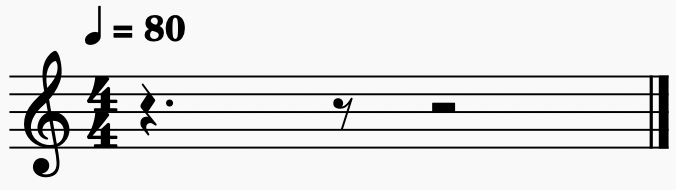
\includegraphics[width=0.38\textwidth]{images/rest}
\caption{Dotted quarter rest}
\end{figure}
\newpage
%--------------------------------------------------------------------------------------------------------------------------------------------------------
\section{Notes}
\label{sec:notes}
The syntax for a note is as follows

\begin{verbatim}
(<NOTENAME><ACCIDENTAL><OCTAVE> <DURATION>)
\end{verbatim}

\noindent where \param{NOTENAME} is taken from one of the following options:
\begin{verbatim}
F,C,G,D,E,A,B
\end{verbatim}

\noindent and \param{ACCIDENTAL} is taken from one of the following options:
\begin{verbatim}
#, ##, b, bb
\end{verbatim}

\param{ACCIDENTAL} is an optional parameter. If the user leaves it out, the note is considered natural. Notice that double sharps are represented with \verb.##. rather than the conventional \musDoubleSharp \; symbol, as this is not an easily typed out character on a keyboard.

\param{OCTAVE} is taken from one of the following options:
\begin{verbatim}
1,2,3,4,5,6,7,8
\end{verbatim}
\noindent as these are the octaves of a standard piano.

\param{DURATION} is taken from the same options as in \Cref{sec:rests}.

Examples of MusAssist notes are \verb.(Cbb5 eighth)., \verb.(D#5 eighth)., and \verb.(A2 quarter).

These expressions,  respectively, translate to the following when compiled and loaded into MuseScore:

\begin{figure}[h!]
\centering
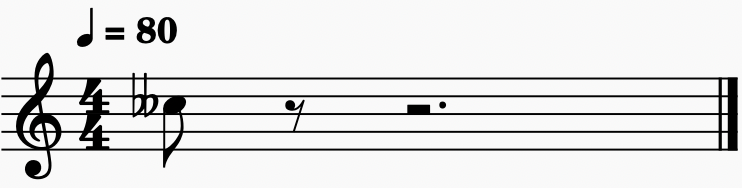
\includegraphics[width=0.38\textwidth]{images/cbb5}
\caption{Eighth note  C\musDoubleFlat5}
\end{figure}

\begin{figure}[h!]
\centering
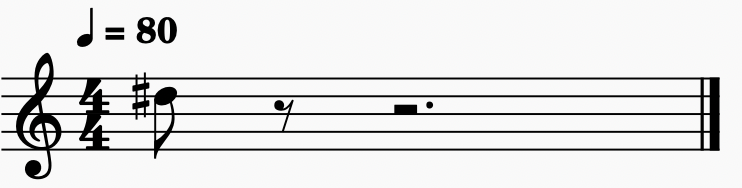
\includegraphics[width=0.38\textwidth]{images/dsharp5}
\caption{Eighth note  D\musSharp5}
\end{figure}

\begin{figure}[h!]
\centering
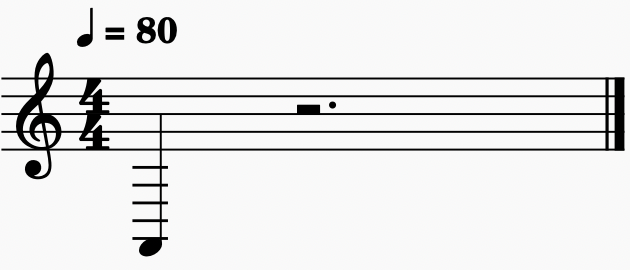
\includegraphics[width=0.38\textwidth]{images/a2}
\caption{Eighth note A2}
\end{figure}

%--------------------------------------------------------------------------------------------------------------------------------------------------------

\section{Custom Chords}
The syntax for a custom chord is as follows

\begin{verbatim}
([<NOTENAME><ACCIDENTAL><OCTAVE>] <DURATION>)
\end{verbatim}

\noindent where \param{NOTENAME}, \param{ACCIDENTAL}, \param{OCTAVE}, and \param{DURATION} are taken from the same options as in \Cref{sec:notes}, and \param{ACCIDENTAL} is similarly optional, with natural implied when it is left out.

\verb.[.\param{NOTENAME}\param{ACCIDENTAL}\param{OCTAVE}\verb.]. indicates an arbitrarily long list supplied by the user, where each of the values are of the form \param{NOTENAME}\param{ACCIDENTAL}\param{OCTAVE}

Examples of MusAssist custom chords are \verb.([Bb5, Dbb6, C5] half). and  \verb.([C##1, E5] sixteenth).

These expressions,  respectively, translate to the following when compiled and loaded into in MuseScore:

\begin{figure}[h!]
\centering
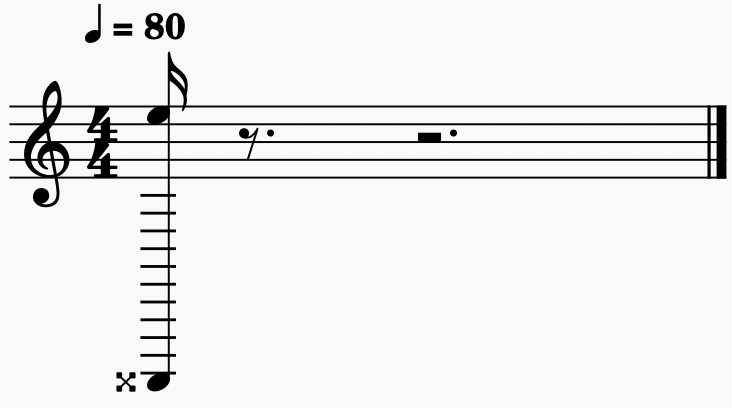
\includegraphics[width=0.38\textwidth]{images/custom1}
\caption{Half note chord with notes B\musFlat6, D\musDoubleFlat6, and C5 }
\end{figure}

\begin{figure}[h!]
\centering
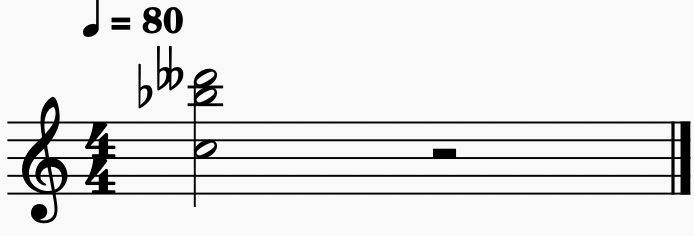
\includegraphics[width=0.38\textwidth]{images/custom2}
\caption{Sixteenth note chord with notes C\musDoubleSharp 1 and E5}
\end{figure}
\newpage
%--------------------------------------------------------------------------------------------------------------------------------------------------------

\section{Chord Templates}
\label{sec:chordtemplatessyntax}
The syntax for a chord template is as follows

\begin{verbatim}
(<NOTENAME><ACCIDENTAL><OCTAVE> <QUALITY> <CHORDTYPE> inv:<INVERSION> <DURATION>)
\end{verbatim}

\noindent where \param{NOTENAME}, \param{ACCIDENTAL}, \param{OCTAVE}, and \param{DURATION} are taken from the same options as in \Cref{sec:notes}, and \param{ACCIDENTAL} is similarly optional, with natural implied when it is left out.

\param{ACCIDENTAL} is now taken from one of the following restricted options:
\begin{verbatim}
#, b
\end{verbatim}
\noindent This is because chords cannot be built on a double sharp or flat, as such chords may introduce triple sharps or flats, and MusAssist does not support these elements. \param{ACCIDENTAL} does continue remain optional, with natural implied when it is left out.


\param{INVERSION} is taken from one of the following options:
\begin{verbatim}
root, first, second, third
\end{verbatim}

\noindent where \verb.third. is only an option for seventh chords.

\param{QUALITY} is taken from one of the following options:
\begin{verbatim}
maj, min, aug, dim, halfdim
\end{verbatim}

\noindent (which, as one would expect, indicate major, minor, augmented, diminished, and half diminished qualities). Half diminished can only apply to a seventh chord, not to triads.


Finally, \param{CHORDTYPE} is taken from one of the following options:
\begin{verbatim}
triad, seventh
\end{verbatim}


Examples of MusAssist harmonic sequences are \verb.(C6 min triad inv:first quarter). and  \\\verb.(F#4 halfdim seventh inv:third eighth).

These expressions,  respectively, translate to the following when compiled and loaded into MuseScore:

\begin{figure}[h!]
\centering
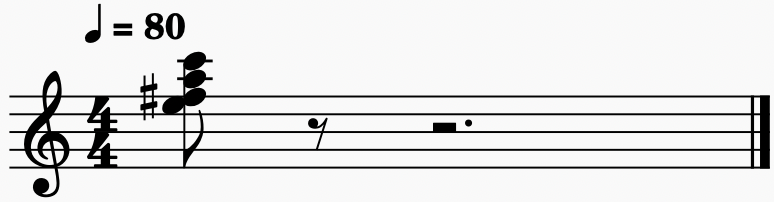
\includegraphics[width=0.38\textwidth]{images/cmintriad}
\caption{C6 minor triad, first inversion}
\end{figure}

\begin{figure}[h!]
\centering
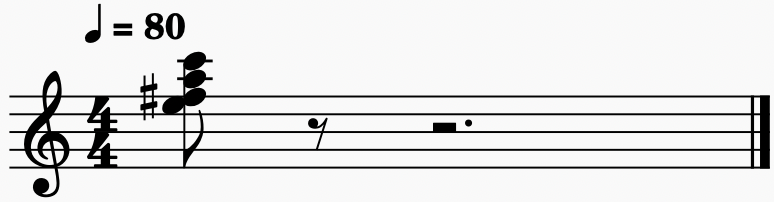
\includegraphics[width=0.38\textwidth]{images/f7}
\caption{F\musSharp4 half diminished seventh, third inversion}
\end{figure}
\newpage
%--------------------------------------------------------------------------------------------------------------------------------------------------------

\section{Harmonic Sequences}
\label{sec:harmseq}
The syntax for a harmonic sequence is as follows

\begin{verbatim}
(<HARMSEQTYPE> <NOTENAME><ACCIDENTAL><OCTAVE> <QUALITY> <DURATION> length:<LENGTH>)
\end{verbatim}

\noindent where \param{NOTENAME}, \param{OCTAVE}, and \param{DURATION} (but not \verb.<ACCIDENTAL>.) are taken from the same options as in \Cref{sec:notes}. \param{DURATION} and \param{LENGTH} are not to be confused: \param{DURATION} specifies the length of each individual  chord in the harmonic sequence, while \param{LENGTH} specifies the number of chords in the sequence. 

Unlike chord templates, here \param{QUALITY} is taken from one of the following restricted options:
\begin{verbatim}
maj, min
\end{verbatim}
\noindent and \param{ACCIDENTAL} is taken from the same restricted options as in \Cref{sec:chordtemplatessyntax}. \param{ACCIDENTAL}  continues remain optional, with natural implied when it is left out.

This is because together, \verb.<NOTENAME><ACCIDENTAL><OCTAVE> <QUALITY>. determine the local key (and the start octave) of the harmonic sequence. A key can only be major or minor, and a key in MusAssist cannot be described with a double sharp or flat, as such key signatures may introduce triple sharps or flats, which recall are not supported. 

%%%%%%%%%%%%%%%%%%%%%%%%%%%%%%%%%%%%%%%%%%%%%%%%%%%%%%%%%%%%
%%%%%%%%%%%%%%%%%%%%%%%%%%%%%%%%%%%%%%%%%%%%%%%%%%%%%%%%%%%%
%%%%%%%%%%%%%%%%%%%%%%%%%%%%%%%%%%%%%%%%%%%%%%%%%%%%%%%%%%%%
%%%%%%%%%%%%%%%%%%%%%%%%%%%%%%%%%%%%%%%%%%%%%%%%%%%%%%%%%%%%
%%%%%%%%%%%%%%%%%%%%%%%%%%%%%%%%%%%%%%%%%%%%%%%%%%%%%%%%%%%%
%NEED TO TALK ABOUT INVALID KEYS WITH DOUBLE ACCIDENTALS!!!!!! this also applies to harmseq and cadences!!!
%%%%%%%%%%%%%%%%%%%%%%%%%%%%%%%%%%%%%%%%%%%%%%%%%%%%%%%%%%%

\param{HARMSEQTYPE} is taken from one of the following options:
\begin{verbatim}
AscFifths, DescFifths, Asc56, Desc56
\end{verbatim}

These are the four most commonly encountered sequences. The musical theoretical aspects of harmonic sequences are outside the scope of this paper, but a good reference for review can be found here: \href{https://myweb.fsu.edu/nrogers/Handouts/Diatonic_Sequence_Handout.pdf}{https://myweb.fsu.edu/nrogers/Handouts/Diatonic\_Sequence\_Handout.pdf}

Finally, \param{LENGTH} is any natural number (though a sequence that is too long will exceed the octave restriction of 1 through 8).

Harmonic sequences can be written out in a variety of ways, depending on the chord inversions chosen. Furthermore, MusAssist at this time does not support multiple clefs (i.e. lines) simultaneously. This means that currently, harmonic sequences cannot be written with a bass line. However, the harmonies are preserved through the upper voices in keyboard-style voice leading. Though the upper-voice harmonization of a harmonic sequence need not follow the direction of the sequence's name (i.e. a descending fifths sequences could present as a series of ascending chords in the upper voices), MusAssist chooses a chord inversion and voice leading pattern such that each sequence does align with the direction of its name. 

The chord progressions of each sequence in MusAssist are summarized in more detail in the following table (all in major, for the sake of example). Each of the four supported harmonic sequences consists of fourteen chords before it repeats (albeit in a different octave), which are as follows:

\begin{table}[h!]
\begin{tabular}{|l|llllllllllllll|}
\hline
Ascending Fifths  & I$^{6 \atop 4}$ & V                & ii$^{6 \atop 4}$ & vi                & iii$^{6 \atop 4}$ & vii$^\text{o}$   & IV$^{6 \atop 4}$ & I               & V$^{6 \atop 4}$             & ii                          & vi$^{6 \atop 4}$ & iii              & vii$^{\text{o}{6 \atop 4}}$ & IV              \\ \hline
Descending Fifths & I               & IV$^{6 \atop 4}$ & vii$^\text{o}$   & iii$^{6 \atop 4}$ & vi                & ii$^{6 \atop 4}$ & V                & I$^{6 \atop 4}$ & IV                          & vii$^{\text{o}{6 \atop 4}}$ & iii              & vi$^{6 \atop 4}$ & ii                          & V$^{6 \atop 4}$ \\ \hline
Ascending 5-6     & I               & vi$^6$           & ii               & vii$^{\text{o}6}$ & iii               & I$^6$            & IV               & ii$^6$          & V                           & iii$^6$                     & vi               & IV$^6$           & vii$^\text{o}$              & V$^6$           \\ \hline
Descending 5-6    & I$^{6 \atop 4}$ & V                & vi$^{6 \atop 4}$ & iii & IV$^{6 \atop 4}$  & I                & ii$^{6 \atop 4}$ & vi              & vii$^{\text{o}{6 \atop 4}}$ & IV                          & V$^{6 \atop 4}$  & ii               & iii$^{6 \atop 4}$           & vii$^\text{o}$  \\ \hline
\end{tabular}
\end{table}

This is demonstrated in each of the following examples, all in C major. Each has length fifteen, to demonstrate the entire 14-chord sequences and also return to the first chord. Principles of smooth voice leading were used for all sequences.

The following figures were created with the following MusAssist expressions, respectively: \\\verb.(AscFifths C4 maj quarter length:15)., \verb.(DescFifths C4 maj quarter length:15)., \\\verb.(Asc56 C4 maj quarter length:15)., \verb.(Desc56 C6 maj quarter length:15).. When compiled and loaded into MuseScore, they look like:

\begin{figure}[h!]
\centering
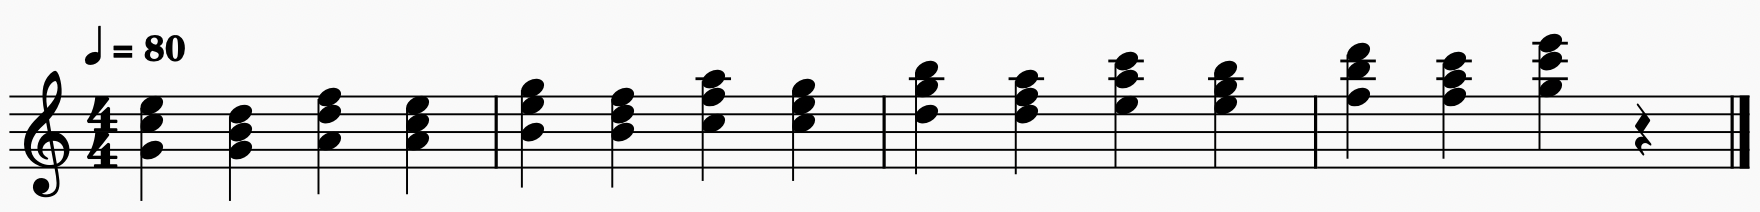
\includegraphics[width=0.5\textwidth]{images/ascfifths}
  \caption{Ascending Fifths Sequence}
  \label{fig:ascfifths}
\end{figure}

\begin{figure}[h!]
\centering
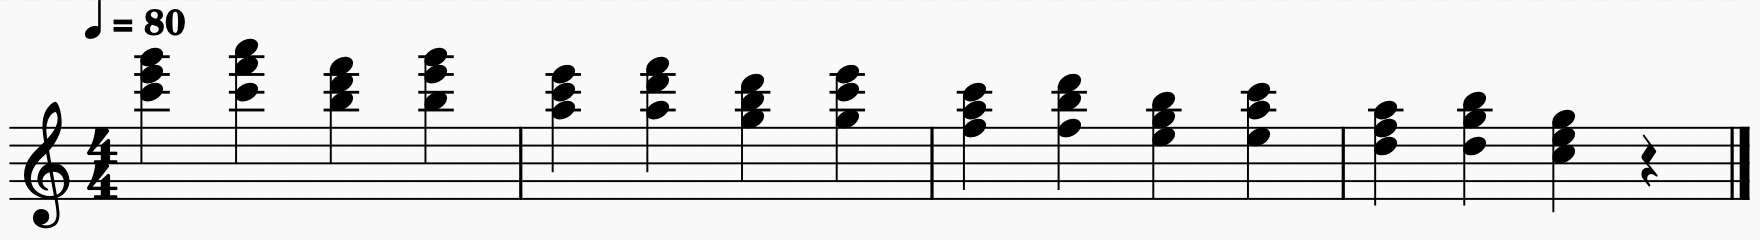
\includegraphics[width=0.5\textwidth]{images/descfifths}
  \caption{Descending Fifths Sequence}
\end{figure}

\begin{figure}[h!]
\centering
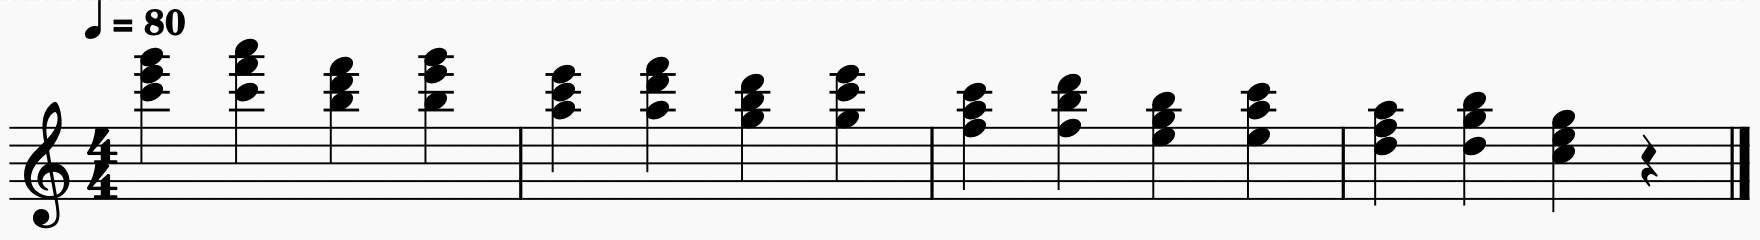
\includegraphics[width=0.5\textwidth]{images/asc56}
  \caption{Ascending 5-6 Sequence}
\end{figure}

\begin{figure}[h!]
\centering
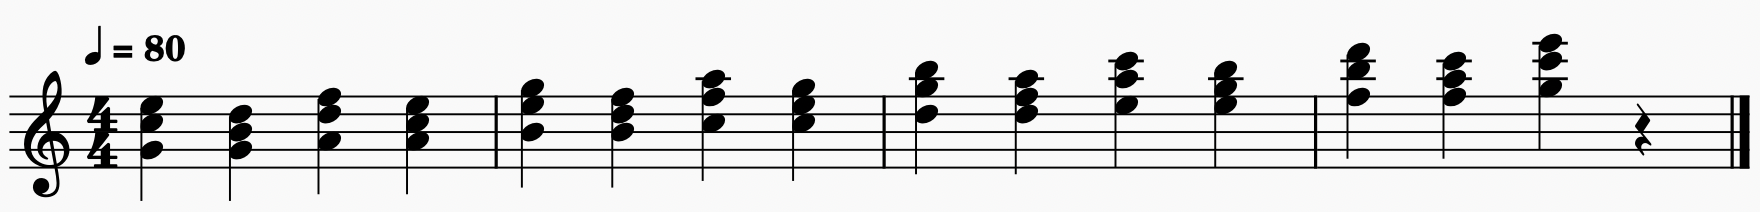
\includegraphics[width=0.5\textwidth]{images/desc56}
  \caption{Descending 5-6 Sequence}
  \label{fig:desc56}
\end{figure}

\newpage

In most music theory settings, the ascending fifths sequence would terminate after five chords (i.e. before it reaches a root position diminished  triad). However, MusAssist does not stop at this chord based on the principle that users should be able to generate sequences of any length. Terminating this sequence after five chords is up to the user.

Furthermore, a minor descending fifths sequence would generally have the final appearance of scale degree seven raised, since it is leading back to the tonic. However, MusAssist does not do this based on the principle that all sequences should follow the pattern they are given, for any arbitrary length. 
%--------------------------------------------------------------------------------------------------------------------------------------------------------

\section{Cadences}

The syntax for a cadence is as follows

\begin{verbatim}
(<CADENCETYPE> <NOTENAME><ACCIDENTAL><OCTAVE> <QUALITY> <DURATION>)
\end{verbatim}

\noindent\param{CADENCETYPE} is taken from one of the following options:
\begin{verbatim}
PerfAuthCadence, ImperfAuthCadence, HalfCadence, PlagalCadence, DeceptiveCadence
\end{verbatim}

\param{NOTENAME}, \param{OCTAVE}, and \param{DURATION} are taken from the same options as in \Cref{sec:notes}. 

\param{ACCIDENTAL} is taken from the same restricted options as in \Cref{sec:chordtemplatessyntax} and \param{QUALITY} is taken from the same restricted options as in \Cref{sec:harmseq}.

\noindent Together, \verb.<NOTENAME><ACCIDENTAL><OCTAVE> <QUALITY>. determine the local key (and the start octave) of the cadences. Recall that a key can only be major or minor, and a key cannot be in a double sharp or flat due to the potential for triple sharps or flats to appear in the key.

%%%%%%%%%%%%%%%%%%%%%%%%%%%%%%%%%%%%%%%%%%%%%%%%%%%%%%%%%%%%
%%%%%%%%%%%%%%%%%%%%%%%%%%%%%%%%%%%%%%%%%%%%%%%%%%%%%%%%%%%%
%%%%%%%%%%%%%%%%%%%%%%%%%%%%%%%%%%%%%%%%%%%%%%%%%%%%%%%%%%%%
%%%%%%%%%%%%%%%%%%%%%%%%%%%%%%%%%%%%%%%%%%%%%%%%%%%%%%%%%%%%
%%%%%%%%%%%%%%%%%%%%%%%%%%%%%%%%%%%%%%%%%%%%%%%%%%%%%%%%%%%%
%NEED TO TALK ABOUT INVALID KEYS WITH DOUBLE ACCIDENTALS!!!!!! this also applies to harmseq and cadences!!!
%%%%%%%%%%%%%%%%%%%%%%%%%%%%%%%%%%%%%%%%%%%%%%%%%%%%%%%%%%%

The music theory of cadences is outside the scope of this paper, but good references for review can be found  here: \href{https://sites.google.com/site/musictheorycheatsheet/diatonicism/ii-functional-harmony-and-cadences}{https://sites.google.com/site/musictheorycheatsheet/diatonicism/ii-functional-harmony-and-cadences} and here: \href{https://sites.google.com/site/musictheorycheatsheet/diatonicism/ii-functional-harmony-and-cadences}{https://sites.google.com/site/musictheorycheatsheet/diatonicism/ii-functional-harmony-and-cadences} 

Again, the cadences are written in the upper voices only, in keyboard voice leading style, due to MusAssist's current lack of support for multiple clefs. Principles of smooth voice leading were applied throughout.

From a music theory standpoint, based on the principles of functional harmony, there are several ways to represent each of these cadences. In MusAssist, the following representations were chosen. The major version is presented first, and the minor version is after that, in parentheses.

\begin{table}[h!]
\begin{tabular}{|l|l|l|l|l|}
\hline
Perfect Authentic & Imperfect Authentic & Plagal & Deceptive & Half \\ \hline
IV-V-I (iv-V-i) 
& IV-vii$^{\text{o}{6 \atop 4}}$-I$^{6 \atop 4}$ (iv-vii$^{\text{o}{6 \atop 4}}$-i$^{6 \atop 4}$)
& IV$^{6 \atop 4}$-I (iv$^{6 \atop 4}$-I)        
& IV-V$^{6 \atop 4}$-vi$^{6 \atop 4}$ (iv-V$^{6 \atop 4}$-VI$^{6 \atop 4}$)
& IV-ii$^6$-V (iv-ii$^{\text{o}6}$-V)
\\ \hline
\end{tabular}
\label{table:cadences}
\end{table}

The five possible cadence types in MusAssist are demonstrated in the following examples. 

\noindent\verb.(PerfAuthCadence Eb5 min sixteenth)., \verb.(ImperfAuthCadence F#5 min quarter)., \\\verb.(DeceptiveCadence B4 maj eighth)., \verb.(HalfCadence G#5 min whole)., \verb.(PlagalCadence C5 maj half).

These MusAssist expressions,  respectively, translate to the following when  compiled and loaded into the MuseScore notation software. Notice the doubled root in the perfect authentic cadence in an attempt to simulate the 4-5-1 bass line, as well as to preserve the 2-1 downward step in the uppermost voice required for this cadence. 
\begin{figure}[h!]
\centering
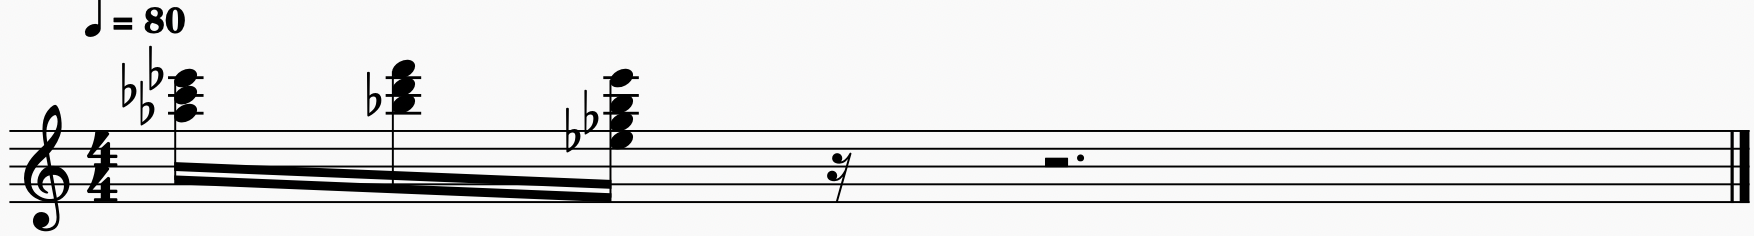
\includegraphics[width=0.7\textwidth]{images/perfauth}
  \caption{Perfect Authentic Cadence in E\musFlat\; minor}
\end{figure}

\begin{figure}[h!]
\centering
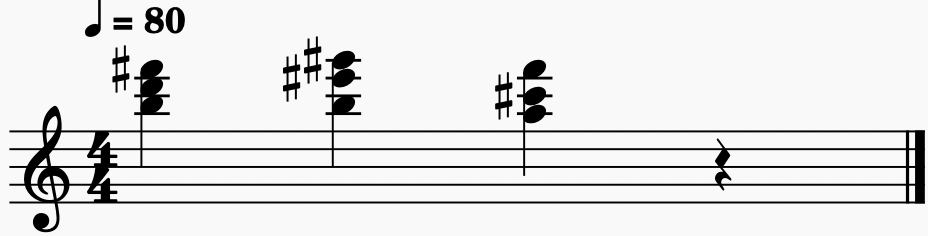
\includegraphics[width=0.5\textwidth]{images/imperfauth}
  \caption{Imperfect Authentic Cadence in F\# minor}
\end{figure}

\begin{figure}[h!]
\centering
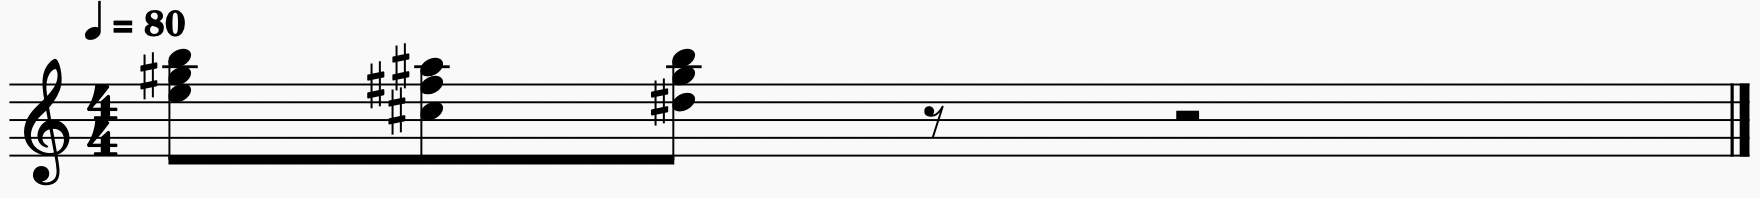
\includegraphics[width=0.7\textwidth]{images/deceptive}
  \caption{Deceptive Cadence in B major}
\end{figure}

\begin{figure}[h!]
\centering
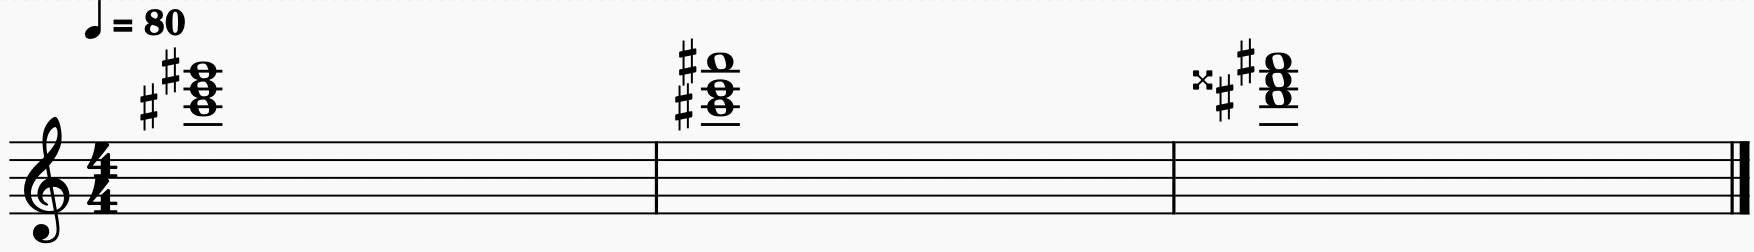
\includegraphics[width=0.7\textwidth]{images/half}
  \caption{Half Cadence in G\# minor}
\end{figure}

\begin{figure}[h!]
\centering
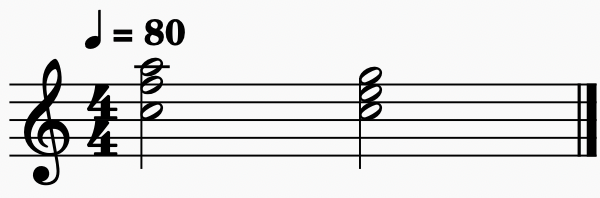
\includegraphics[width=0.3\textwidth]{images/plagal}
  \caption{Plagal Cadence in C major}
\end{figure}

%--------------------------------------------------------------------------------------------------------------------------------------------------------

\section{Labeled Expressions}
\label{sec:labels}
A series of any of the above MusAssist expressions can be stored in a label (i.e. a string of the user's choice). The label must start with a letter, and can contain letters, numbers, underscores, and single quotes. This label is thus syntactic sugar for the musical expressions it refers to. When the label is referenced later in the program, the compiler will translate the expression it refers to. 

For example,
\begin{verbatim}
label123_' = (D4 whole) (Ab4 quarter) (rest whole) ([Bbb5, Db5, C5] half) 
label123_'
\end{verbatim}

will translate to the following when compiled and loaded into MuseScore:

\begin{figure}[h!]
\centering
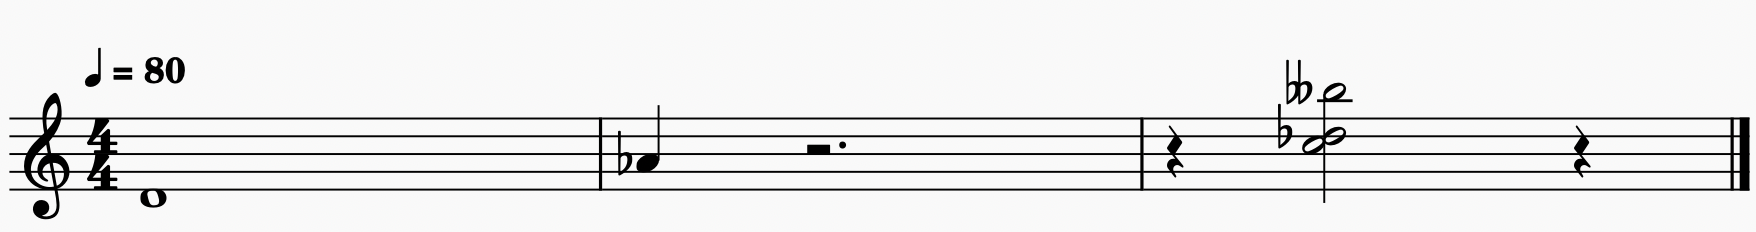
\includegraphics[width=0.7\textwidth]{images/label}
  \caption{Music Translated from Labeled Expression}
\end{figure}

%--------------------------------------------------------------------------------------------------------------------------------------------------------

\section{Key Signatures}

The syntax for a key signature change is as follows

\begin{verbatim}
SET_KEY <NOTENAME><ACCIDENTAL><QUALITY>
\end{verbatim}

\noindent where \param{NOTENAME} is taken from the same options as in \Cref{sec:notes}, \param{ACCIDENTAL} is taken from the same restricted options as in \Cref{sec:chordtemplatessyntax} and \param{QUALITY} is taken from the same restricted options as in \Cref{sec:harmseq}. Again, accidentals and qualities are restricted because keys must be major or minor, and cannot be built on a double sharp or flat due to the problem of such keys introducing triple sharps or flats.

A key signature also cannot have double sharps or flats, which could happen even if the key signature is not built on a double sharp or flat note. This means that the following key signatures, though they are built on seemingly valid notes, are actually invalid:
\begin{verbatim}
D#maj, E#maj, G#maj, A#maj, B#maj, Fbmaj
E#min, B#min, Cbmin, Dbmin, Fbmin, Gbmin
\end{verbatim}

%%%%%%%%%%%%%%%%%%%%%%%%%%%%%%%%%%%%%%%%%%%%%%%%%%%%%%%%%%%%
%%%%%%%%%%%%%%%%%%%%%%%%%%%%%%%%%%%%%%%%%%%%%%%%%%%%%%%%%%%%
%%%%%%%%%%%%%%%%%%%%%%%%%%%%%%%%%%%%%%%%%%%%%%%%%%%%%%%%%%%%
%%%%%%%%%%%%%%%%%%%%%%%%%%%%%%%%%%%%%%%%%%%%%%%%%%%%%%%%%%%%
%%%%%%%%%%%%%%%%%%%%%%%%%%%%%%%%%%%%%%%%%%%%%%%%%%%%%%%%%%%%
%NEED TO TALK ABOUT INVALID KEYS WITH DOUBLE ACCIDENTALS!!!!!! this also applies to harmseq and cadences!!!
%%%%%%%%%%%%%%%%%%%%%%%%%%%%%%%%%%%%%%%%%%%%%%%%%%%%%%%%%%%

Notably, keys cannot be changed within a measure. If the users attempts to do this, a new measure will automatically get started. Also, a MusAssist key signature change must occur by itself on its own line. Finally, if the user sets a key signature to what the current key signature already is, nothing will happen. 

For example,
\begin{verbatim}
SET_KEY Dmin
SET_KEY Amaj
SET_KEY Amaj
SET_KEY Cmaj
\end{verbatim}

will translate to the following when compiled and loaded into MuseScore:

\begin{figure}[h!]
\centering
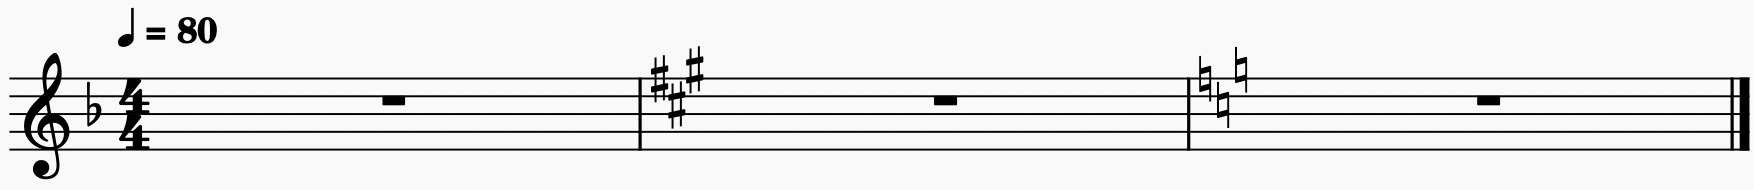
\includegraphics[width=0.7\textwidth]{images/keys}
  \caption{Key Signature Changes}
\end{figure}
\newpage
%--------------------------------------------------------------------------------------------------------------------------------------------------------

\section{New Measures}
A new measure can be started at any point in the program with the command \verb.NEW_MEASURE.

For example,
\begin{verbatim}
(D4 quarter)
NEW_MEASURE
(E4 eighth)
\end{verbatim}

will translate to the following when compiled and loaded into MuseScore:

\begin{figure}[h!]
\centering
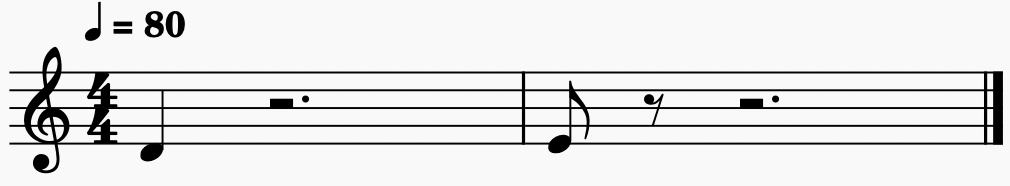
\includegraphics[width=0.5\textwidth]{images/newmeasure}
  \caption{Starting a New Measure}
\end{figure}

A new measure MusAssist instruction must occur by itself on its own line.

%%%%%%%%%%%%%%%%%%%%%%%%%%%%%%%%%%%%%%%%%%%%%%%%%%%%%%%%%%%%
% add example about consecutive NEW_MEASURE s
\section{Comments}
Comments are designated with \verb.//.. Any text after the comment indicator is ignored by the complier. For instance:\\ \verb.// this is a comment.

MusAssist also supports multiline comments. Any text enclosed between the multiline comment symbols \verb.//*. and \verb.*//. is ignored by the compiler. For instance:
\begin{verbatim}
//* This 
is 
a 
comment *//
\end{verbatim}


%-----------------------------------------------------------------------------------------------------------------------------------------------------------------------------------------------------------------------------------------------------------
%-----------------------------------------------------------------------------------------------------------------------------------------------------------------------------------------------------------------------------------------------------------
\chapter{Lexing and Parsing}

Parsing of MusAssist concrete syntax was implemented with parser combinators using parsers from Parsec, an industrial strength parser library. Parsec's helper module Token was used for lexing. To combine parsers, Haskell's Applicative module was used, and the following custom monadic sequencing operators\footnote{credit: Ben Wiedermann}
\begin{verbatim}
infixl 1 >>=:
left >>=: f = f <$> left

infixl 1 >>:
left >>: v = left >> return v
\end{verbatim}

were defined to generate the results of the parse.

The following sections discuss the parsing of the concrete syntax from \Cref{chap:langfeatures} into abstract syntax. The abstract syntax was carefully designed to best model musical structures organically. MusAssist's parser can be found \href{https://github.com/ilanashapiro/MusAssist/blob/main/app/Parser.hs}{here}, and its abstract  syntax can be found \href{https://github.com/ilanashapiro/MusAssist/blob/main/app/MusAssistAST.hs}{here}.
%--------------------------------------------------------------------------------------------------------------------------------------------------------
\section{Note Names}
Recall from \Cref{sec:notes} that the set of all possible values for the concrete syntax \param{NOTENAME} is:
\begin{verbatim}
F,C,G,D,E,A,B
\end{verbatim}

These are parsed, respectively, into the abstract syntax \verb.NoteName. (a custom Haskell algebraic data type, or ADT, defined as follows:
\newpage
\begin{verbatim}
data NoteName = 
    F
    | C
    | G 
    | D 
    | E 
    | A 
    | B
\end{verbatim}

The reason that an ADT was created for note names, rather than a simple type alias for String, was so that (1) correctness could be enforced for the possible note names and (2) so that custom orderings, as well as the ability to take  successors and predecessors, can be defined for the note names. As will be discussed in \Cref{chap:ir}, two orderings will be needed for note names, which are accomplished through deriving \verb.Ord. and also implementing a custom instance of the \verb.Enum. typeclass. For now, simply notice that the \verb.NoteName. ADT lists the notes in the order of sharps.
%--------------------------------------------------------------------------------------------------------------------------------------------------------
\section{Accidentals}
Recall from \Cref{sec:notes} that the set of all possible values for the concrete syntax \param{ACCIDENTAL} is:
\begin{verbatim}
#, ##, b, bb
\end{verbatim}

These are parsed into the abstract syntax \verb.Accidental. (a custom Haskell ADT) defined below. Recall that \param{ACCIDENTAL} is always an optional parameter in the  concrete syntax. The mappings from concrete to abstract syntax are as one would expect semantically, and when the user leaves out the \param{ACCIDENTAL} parameter after \param{NOTENAME}, the result of the parse is \verb.Natural..

\begin{verbatim}
data Accidental = 
     DoubleFlat 
     | Flat 
     | Natural
     | Sharp
     | DoubleSharp
\end{verbatim}

Like notes, accidentals were not represented in the abstract syntax with a String alias in order to (1) enforce correctness for the limited possible values and (2) enforce a custom ordering. As will be discussed in \Cref{sec:chordtemplates}, one ordering (as well as the ability to take successors and predecessors) will be needed for accidentals, which is accomplished through deriving \verb.Enum..
%--------------------------------------------------------------------------------------------------------------------------------------------------------
\section{Octaves}
Recall from \Cref{sec:notes} that the set of all possible values for the concrete syntax \param{OCTAVE} is:
\begin{verbatim}
1,2,3,4,5,6,7,8
\end{verbatim}

These are parsed into the abstract syntax \verb.Octave., a Haskell type alias for Int. \verb.Octave. is defined as follows:

\begin{verbatim}
type Octave = Int
\end{verbatim}

An Int type alias, rather than a custom ADT, was chosen for octaves as the constraint of  1-8 is simple to enforce in a later stage, and no custom ordering is needed beyond what is already provided by Int.
%--------------------------------------------------------------------------------------------------------------------------------------------------------
\section{Inversions}
Recall from \Cref{sec:chordtemplatessyntax} that the set of all possible values for the concrete syntax \param{INVERSION} is:
\begin{verbatim}
root, first, second, third
\end{verbatim}

They are parsed, respectively, into the abstract syntax \verb.Inversion., a custom Haskell ADT. \verb.Inversion. is defined as follows:

\begin{verbatim}
data Inversion = 
  Root 
  | First 
  | Second 
  | Third
\end{verbatim}

An ADT was better than a String alias to represent inversions in order to best enforce correctness of the data given their limited possible values. 

%--------------------------------------------------------------------------------------------------------------------------------------------------------
\section{Length}

Recall from \Cref{sec:harmseq} that the concrete syntax \param{LENGTH} can be any natural number. This thus parses to the abstract syntax \verb.Length., a Haskell type alias for Int:

\begin{verbatim}
type Length = Int
\end{verbatim}
 
%--------------------------------------------------------------------------------------------------------------------------------------------------------
\section{Labels}
Recall from \Cref{sec:labels} that a the concrete syntax of a MusAssist label is simply a string of the user's choice that must start with a letter, and can contain letters, numbers, underscores, and single quotes. Labels thus parse to the abstract syntax \verb.Label., a Haskell type alias for String:

\begin{verbatim}
type Label = String
\end{verbatim}

%--------------------------------------------------------------------------------------------------------------------------------------------------------
\section{Durations}
Recall from \Cref{sec:rests} that the set of all possible values for the concrete syntax \param{DURATION} is:

\begin{verbatim}
sixteenth, eighth, dotted_eighth, quarter, dotted_quarter, half, dotted_half, whole
\end{verbatim}

They are parsed, respectively, into the abstract syntax \verb.Duration., a custom Haskell ADT. \verb.Duration. is defined as follows:

\begin{verbatim}
data Duration = 
    Sixteenth
    | Eighth 
    | DottedEighth 
    | Quarter 
    | DottedQuarter 
    | DottedHalf 
    | Half 
    | Whole 
\end{verbatim}

Durations were not represented in the abstract syntax with a String alias in order to (1) enforce correctness for the limited possible values and (2) enforce a custom ordering. \verb.Duration. derives \verb.Ord., which enforces the ordering of durations from smallest to largest, as seen in the data definition. Of note, durations are not represented as floats as MusAssist does not support arbitrarily complex durations, and ordered custom data types are easier to work with than floats.

%--------------------------------------------------------------------------------------------------------------------------------------------------------
\section{Qualities}

Recall from \Cref{sec:chordtemplates}  that the set of all possible values for the concrete syntax \param{QUALITY} is:
\begin{verbatim}
maj, min, aug, dim, halfdim
\end{verbatim}

They are parsed, respectively, into the abstract syntax \verb.Quality., a custom Haskell ADT. \verb.Quality. is defined as follows:

\begin{verbatim}
data Quality = 
    Major 
    | Minor
    | Augmented 
    | Diminished
    | HalfDiminished
\end{verbatim}

An ADT was better than a String alias to represent qualities in order to best enforce correctness of the data given their limited possible values. 
%--------------------------------------------------------------------------------------------------------------------------------------------------------
\section{Chord Types}

Recall from \Cref{sec:chordtemplates}  that the set of all possible values for the concrete syntax \param{CHORDTYPE} is:
\begin{verbatim}
triad, seventh
\end{verbatim}

They are parsed, respectively, into the abstract syntax \verb.ChordType., a custom Haskell ADT. \verb.ChordType. is defined as follows:

\begin{verbatim}
data ChordType = 
     Triad 
     | Seventh
\end{verbatim}

An ADT was better than a String alias to represent qualities in order to best enforce correctness of the data given their limited possible values. 

%--------------------------------------------------------------------------------------------------------------------------------------------------------
\section{Cadence Types}

Recall from \Cref{sec:chordtemplates}  that the set of all possible values for the concrete syntax \param{CADENCETYPE} is:
\begin{verbatim}
PerfAuthCadence, ImperfAuthCadence, HalfCadence, PlagalCadence, DeceptiveCadence
\end{verbatim}

They are parsed, respectively, into the abstract syntax \verb.CadenceType., a custom Haskell ADT. \verb.CadenceType. is defined as follows:

\begin{verbatim}
data CadenceType = 
  PerfAuth 
  | ImperfAuth
  | Plagal
  | HalfCad
  | Deceptive
\end{verbatim}

An ADT was better than a String alias to represent cadence types in order to best enforce correctness of the data given their limited possible values. 

%--------------------------------------------------------------------------------------------------------------------------------------------------------
\section{Harmonic Sequence Types}
Recall from \Cref{sec:harmseq}  that the set of all possible values for the concrete syntax \param{HARMSEQTYPE} is:

\begin{verbatim}
AscFifths, DescFifths, Asc56, Desc56
\end{verbatim}

They are parsed, respectively, into the abstract syntax \verb.HarmonicSequenceType., a custom Haskell ADT. \verb.HarmonicSequenceType. is defined as follows:

\begin{verbatim}
data HarmonicSequenceType = 
  AscFifths
  | DescFifths
  | Asc56 
  | Desc56
\end{verbatim}

An ADT was better than a String alias to represent harmonic sequence types in order to best enforce correctness of the data given their limited possible values. 
%--------------------------------------------------------------------------------------------------------------------------------------------------------
\section{Tones}
\label{sec:tones}

A tone (i.e. a ``sounding," or non-rest, note) is comprised of a note name, accidental, and octave, and is represented with \verb.Tone., a custom Haskell ADT:

\begin{verbatim}
data Tone = Tone NoteName Accidental Octave 
\end{verbatim}

The parsers for note name, accidental, and octave are thus combined to create a parser for tones:

\begin{verbatim}
parseTone :: Parsec String () Tone 
parseTone = Tone <$> parseNoteName <*> parseAccidental <*> 
		            (natural >>=: \octave -> fromIntegral octave)
\end{verbatim}
where \verb.natural. is a helper lexing function for natural numbers from Parsec's \verb.Token. module.

%--------------------------------------------------------------------------------------------------------------------------------------------------------
\section{Intermediate Expressions}

An intermediate expression describes one of two entities: a musical template that will get expanded in \Cref{chap:ir}, or a ``final expression" that will not get expanded. Intermediate expressions are represented with \verb.IntermediateExpr., a custom Haskell ADT:

\begin{verbatim}
data IntermediateExpr = 
  Note Tone Duration
  | ChordTemplate Tone Quality ChordType Inversion Duration
  | Cadence CadenceType Tone Quality Duration
  | HarmonicSequence HarmonicSequenceType Tone Quality Duration Length 
  | Label Label
  | FinalExpr Expr
\end{verbatim}

Parsers for the musical building blocks described in the previous sections of this chapter are combined, similar to \Cref{sec:tones}, to create parsers for each \verb.IntermediateExpr.

As the ADT demonstrates, the templates to expand are notes, chord templates, cadence, harmonic sequences, and labels. In \Cref{chap:ir}, they will be each expanded to a value of type \verb.Expr., a custom Haskell ADT describing the building blocks of all musical expressions:

\begin{verbatim}
data Expr = 
  Rest Duration
  | Chord [Tone] Duration
  | LabeledExpr [Expr]
\end{verbatim}

Any template described in \verb.IntermediateExpr. will get expanded to the \verb.Expr.s it contains. Another way of thinking about this is that \verb.IntermediateExpr.s get ``lowered" to \verb.Expr.s.

An \verb.IntermediateExpr. of type \verb.FinalExpr. is simply unwrapped to the \verb.Expr. it contains. The concrete syntax that parses to \verb.FinalExpr. is that for rests and custom chords. 

%--------------------------------------------------------------------------------------------------------------------------------------------------------
\section{Intermediate Instructions}

An intermediate instruction describes the four possible instructions in a MusAssist program: changing the key signature, creating a new measure, writing a series of musical expressions, or assigning a label to a series of expressions to be reused later. Intermediate instructions are represented with \verb.IntermediateInstr., a custom Haskell ADT:

\begin{verbatim}
data IntermediateInstr = 
  IRKeySignature NoteName Accidental Quality
  | IRNewMeasure
  | IRWrite [IntermediateExpr]
  | IRAssign Label [IntermediateExpr]
\end{verbatim}

As will be discussed in \Cref{chap:ir}, each \verb.IntermediateInstr. is expanded in the intermediate representations phase to a value in the ADT \verb.Instr.:

\begin{verbatim}
data Instr = 
  KeySignature Int Int 
  | NewMeasure 
  | Write [Expr]
  | Assign Label [Expr] 
\end{verbatim}

Like \verb.Expr., \verb.Instr. is not included in the parse result. \verb.IRKeySignature. is a template describing a key signature that gets expanded (or ``lowered") from its description to the number of sharps and flats held in \verb.KeySignature. Every other \verb.IntermediateInstr. simply maps 1-1 to its corresponding \verb.Instr., with \verb.IntermediateExpr. parameters expanded to \verb.Expr. as necessary. Again, this will be explained in great detail in \Cref{chap:ir}.

%--------------------------------------------------------------------------------------------------------------------------------------------------------
\section{Final Remarks}
\label{sec:finalremarks}

When writing the parser, it was important to order parser alternatives correctly due to the issue of overlapping prefixes of identifiers in the concrete syntax. For instance, consider the parser for intermediate expressions (i.e. that maps to the ADT \verb.IntermediateExpr.)

\begin{verbatim}
parseExpr :: Parsec String () IntermediateExpr
parseExpr = 
  try parseLabel
  <|> parens 
    (try parseChordTemplate 
      <|> try parseNote
      <|> try parseCadence
      <|> parseFinalExpr
      <|> parseHarmSeq)
    <?> "Expected expression"
\end{verbatim}

We must call \verb.parseChordTemplate. before \verb.parseNote., because \verb.parseChordTemplate. will attempt to parse the string ``halfdim" (i.e. a quality) and parseNote will attempt to parse the string ``half" (i.e. a duration). Since ``half" is a prefix of ``halfdim", this means that if we call parseNote before parseChordTemplate on the string ``halfdim," the parse will succeed on the prefix ``half", which will incorrectly be parsed as a duration, and then the parse will fail on ``dim." Furthermore, as seen in \verb.parseExpr., it is necessary to use Parsec's ``try" keyword on all parsers that succeed on strings with overlapping prefixes, even when they are in the right order, so that when the parse fails on the first parser alternative(s) after the overlapping prefix, no input will get consumed before trying the next one.

%--------------------------------------------------------------------------------------------------------------------------------------------------------
%--------------------------------------------------------------------------------------------------------------------------------------------------------
\chapter{Intermediate Representations}
\label{chap:ir}
This chapter discusses the expansions (or ``lowerings") of the musical templates described in the ADTs \verb.IntermediateInstr. and \verb.IntermediateExpr.. The code for the expansions can be found \href{https://github.com/ilanashapiro/MusAssist/blob/main/app/IRConversion.hs}{here}

%--------------------------------------------------------------------------------------------------------------------------------------------------------
\section{Intermediate Instructions}
The intermediate instructions \verb.IRNewMeasure, IRWrite [IntermediateExpr],. and \\\verb.IRAssign Label [IntermediateExpr]. all have straightforward conversions to \verb.Instr.. 

\verb.IRNewMeasure. simply gets translated to \verb.NewMeasure., \verb.IRWrite [IntermediateExpr]. gets translated to \verb.Write [Expr]., and \verb.IRAssign Label [IntermediateExpr]. gets translated to \verb.Assign Label [Expr]. (The expansion of the \verb.IntermediateExpr.s in the lists is discussed in \Cref{sec:irexpr}). 

The only complex expansion of an \verb.IntermediateInstr. in the conversion of a key signature description (i.e. note name, accidental, and quality) to the number of sharps or flats in the key.

The expansion of template instructions occurs in \verb.expandIntermediateInstr.
%--------------------------------------------------------------------------------------------------------------------------------------------------------
\subsection{Key Signatures}
The logic for the number of sharps or flats in a key signature is divided based on the two possible key signature qualities: major and minor. 
\subsubsection{Major}

In order to determine the number of sharps or flats for a major key, the possible valid keys (i.e. keys with 0-7 sharps or flats) were listed and divided into keys with 0 or more sharps (\Cref{major_sharp_keys}), and keys with 0 or more flats (\Cref{major_flat_keys}). (If an invalid key is given, an error is thrown).

\begin{figure}[h!]
\centering
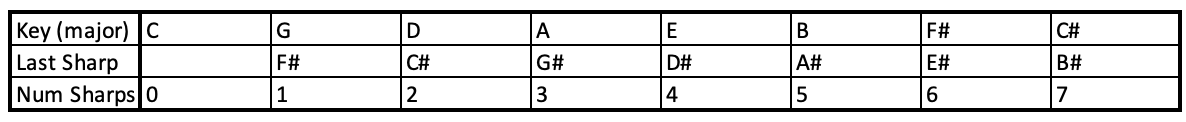
\includegraphics[width=0.9\textwidth]{images/major_sharp}
\caption{Major Keys with 0-7 Sharps}
\label{major_sharp_keys}
\end{figure}

\begin{figure}[h!]
\centering
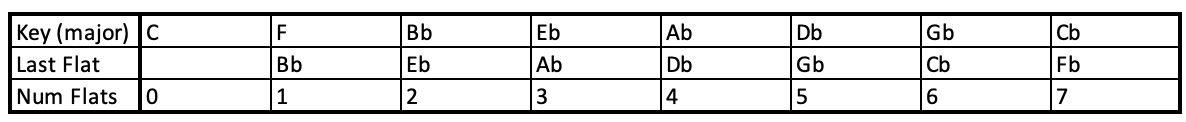
\includegraphics[width=0.9\textwidth]{images/major_flat}
\caption{Major Keys with 0-7 Flats}
\label{major_flat_keys}
\end{figure}

\newpage

Let a \textit{flat key signature} have at least one flat, and let a \textit{sharp key signature} have at least one sharp.

In \Cref{major_sharp_keys}, we see that the number of sharps in a sharp major key signature corresponds to the $index$ of the note name of last sharp appearing in the key signature, in the order of sharps. 

Similarly, in \Cref{major_flat_keys}, we see that the number of flats in a flat major key signature corresponds to $7-(i-1)$, where $i$ is the index of the key signature's note name in the order of sharps. The ``seven-minus" calculation comes from the fact that the order of flats (BEADGCF) is simply the reverse of the order of sharps (FCGDAEB), and there are seven possible sharps or flats because there are seven possible note names. 

In order to support this logic, a list of \verb.NoteNames. in the order of sharps called \verb.globalOrderOfSharps. was created.

The question now becomes how to determine the last sharp in a sharp major key signature. The first step is to determine which key signatures are flat or sharp, given only the key signature's description of note name and accidental. Examining Figures \ref{major_sharp_keys} and \ref{major_flat_keys} again, we notice the following patterns:
\begin{enumerate}
\item  Any key  signature with a flat in its name (i.e. A\musFlat \; major) is a flat key signature. However, the only valid key signatures with flats in their names (i.e. those that do not have double sharps or flats and thus appear in Figures \ref{major_sharp_keys} and \ref{major_flat_keys}) are those whose note name $n$ satisfies $n \geq $\;C in the order of sharps.
\item  Any key  signature with a sharp in its name (i.e. C\musSharp \; major) is a sharp key signature. However, the only valid key signatures with sharps in their names (i.e. those that do not have double sharps or flats and thus appear in Figures \ref{major_sharp_keys} and \ref{major_flat_keys}) are those whose note name $n$ satisfies $n \leq $\;C in the order of sharps.
\item  C major and F major are special cases. C major has zero sharps or flats, and F  major has one flat.
\item  Any other key signature (which must have a natural in its name, i.e. G major) is a sharp key signature.
\end{enumerate}

If we are in a sharp key signature, the rule from music theory is that the last sharp is half a step down from the tonic (i.e. key) note name. However, to determine the name of the note below a given note, we must define a second ordering of the ADT \verb.NoteName.. Recall that \verb.NoteName. already derives \verb.Ord., but uses the order of sharps for this. Thus, to order note names in the order they occur in a scale (i.e. CDEFGAB), we create a custom instance of the \verb.Enum. typeclass for \verb.NoteName. (see: \href{https://github.com/ilanashapiro/MusAssist/blob/main/app/MusAssistAST.hs#L21}{here}). Notably, making \verb.NoteName. an instance of \verb.Enum. does not define a second set of comparison definitions that defy \verb.NoteName.'s derivation of \verb.Ord. (i.e. F is still less than C), but it gives us access to the functions \verb.succ. and \verb.pred. that will return the previous or next \verb.NoteName. based on the scale ordering CDEFGAB. In \verb.NoteName.'s custom instance of \verb.Enum., \verb.succ. and \verb.pred. are both defined circularly. Thus, \verb.succ B. is C, and \verb.pred C. is B.

Thus, if we are in a sharp key signature, to determine the name of the last sharp in the key, we can simply call \verb.pred. on the tonic (i.e. key) note name. To get the index of this resulting \verb.NoteName. in the order of sharps, we simply look up its index in the list \verb.globalOrderOfSharps. (accounting of course for the zero-indexing of lists).

To summarize, the logic of determining the number of sharps or flats in a major key is:
\begin{enumerate}
\item Any key  signature with a flat in its name, and whose note name $n$ satisfies $n \geq $\;C in the order of sharps, is a valid flat key signature. We look up the index of $n$ in \verb.globalOrderOfSharps. (accounting for the zero-indexing of \verb.globalOrderOfSharps.) to get $i$, and the key thus has $7-(i-1)$ flats.
\item Any key  signature with a sharp in its name, and whose note name $n$ satisfies $n \leq $\;C in the order of sharps, is a valid sharp key signature. \verb.pred n. gives us $n'$, the note name of the last sharp in the key signature. The index of $n'$ in \verb.globalOrderOfSharps. tells us how many sharps the key signature has (accounting for the zero-indexing of \verb.globalOrderOfSharps.)

\item Any key  signature with a natural in its name is a key signature. C major (zero sharps or flats) and F major (one flat) are special cases. All other such key signatures are sharp key signatures, and the number of sharps is determined in the same way as just discussed.
\end{enumerate}

%--------------------------------------------------------------------------------------------------------------------------------------------------------
\subsubsection{Minor}
Rather than go through the logic of determining the number of sharps or flats in a minor key signature, we convert each minor key signature to its relative major, and apply the logic from the previous section.

Consider the following mapping of valid minor key signatures (i.e. those without double sharps or flats) to their relative major key signatures. Recall that to get the relative major of a minor key, we go up a minor third in from the tonic of the minor key. 

\begin{figure}[h!]
\centering
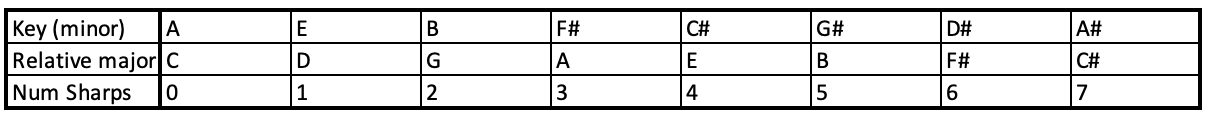
\includegraphics[width=0.9\textwidth]{images/minor_sharp}
\caption{Relative Major Name Accidentals of Minor Keys with Sharp in Name}
\label{minor_sharp}
\end{figure}


\begin{figure}[h!]
\centering
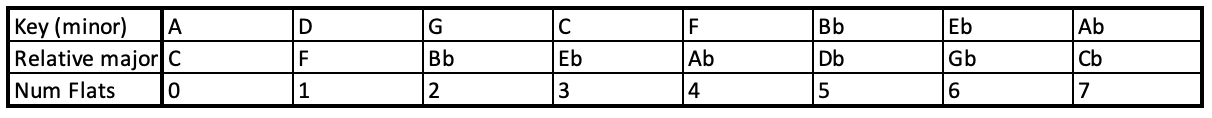
\includegraphics[width=0.9\textwidth]{images/minor_flat}
\caption{Relative Major Name Accidentals of Minor Keys with Sharp in Name}
\label{minor_flat}
\end{figure}
\newpage

This allows us to notice the following patterns. Each of the following diagrams shows the accidental in the name of the relative major key signature of each of the minor keys in the list. Notice that the minor keys are ordered in the order of sharps. 

\begin{figure}[h!]
\centering
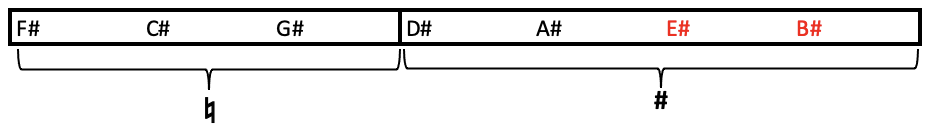
\includegraphics[width=0.9\textwidth]{images/sharp_min_to_maj}
\caption{Relative Major Accidentals for Minor Keys with Sharp in Name}
\label{major_sharp}
\end{figure}

\begin{figure}[h!]
\centering
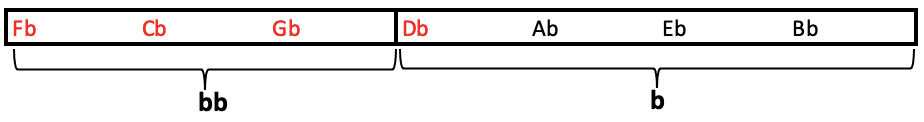
\includegraphics[width=0.9\textwidth]{images/flat_min_to_maj}
\caption{Relative Major Accidentals for Minor Keys with Flat in Name}
\label{major_flat}
\end{figure}

\begin{figure}[h!]
\centering
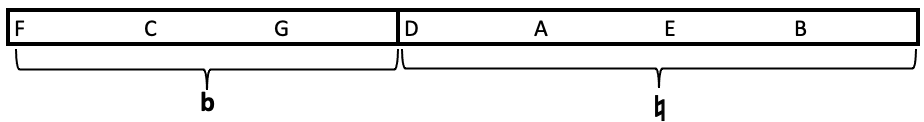
\includegraphics[width=0.9\textwidth]{images/natural_min_to_maj}
\caption{Relative Major Accidentals for Minor Keys with Natural in Name}
\label{major_flat}
\end{figure}

Minor keys in red are invalid (i.e. contain double sharps or flats). However, these will be identified as invalid later, when they have subsequently been processed as major keys after being converted to the relative major. Thus, we can simply determine the accidental of the relative major key by ignoring invalid keys for now. Given a minor key with note name $n$ and accidental $a$, the accidental of its relative major can be determined by D as a ``pivot." 

\begin{enumerate}
\item If $a=\musFlat$, then if $n \geq$ D in the order of sharps, the accidental of its relative major is \musSharp. Otherwise, it is \musNatural.
\item If $a=\musFlat$, then if $n \geq$ D in the order of sharps, the accidental of its relative major is \musFlat. Otherwise, it is \musDoubleFlat.
\item If $a=\musFlat$, then if $n \geq$ D in the order of sharps, the accidental of its relative major is \musNatural. Otherwise, it is \musFlat.
\end{enumerate}

Finally, since we go up a minor third from $n$, the tonic of the minor key, to get  the note name of the relative major, we simply call \verb.succ. twice on $n$ to get the note name of the relative major.

%--------------------------------------------------------------------------------------------------------------------------------------------------------
\section{Intermediate Expressions}
\label{sec:irexpr}

The intermediate expressions \verb.FinalExpr Expr., \verb.Note Tone Duration., \verb.Label Label. have relatively simple expansions. 

For \verb.FinalExpr.s, the \verb.Expr. parameter is simply returned (think of this as ``unwrapping" \verb.FinalExpr Expr.). 

A \verb.Note. will get expanded to a single-tone \verb.Chord..

In terms of \verb.Label.s, when the intermediate instruction \verb.IRAssign Label [IntermediateExpr]. gets translated to the  intermediate instruction \verb.Assign Label [Expr]., the list of expanded \verb.Expr.s is stored in a symbol table mapped to the label name. Then, when expanding \verb.Label., the label name is simply queried in the symbol table, and the list of expanded expressions for that label is returned to replace the label reference. This desugaring step must occur in the intermediate representations stage of the compiler rather than the code generation stage for reasons that will be discussed in \Cref{chap:codegen}.

All the other templates described in \verb.IntermediateExpr. have more complex expansions. On a high level, a \verb.ChordTemplate. will get expanded to a multi-note \verb.Chord., and \verb.Cadence. and a \verb.HarmonicSequence. each will get expanded to a list of multi-note \verb.Chord.s.

The expansion of template expressions occurs in \verb.expandIntermediateExpr..

%--------------------------------------------------------------------------------------------------------------------------------------------------------
\subsection{Chord Templates}
\label{sec:chordtemplates}
Recall that a chord template contains information about its root note, quality, type, inversion, and duration. It will get expanded to the list of notes (i.e. tones) that it describes.

Expansion of chord templates begins with validity checks: that (1) the chord root is not a double sharp or flat (MusAssist does not support this), and (2) that the chord is not a half diminished triad (impossible according to music theory). After this, each of the notes of the chord are determined.

To do this, a helper function called \verb.generateToneWithinScale. was created. This function, given the tonic tone and quality (either major or minor), will generate the tone within that diatonic scale given the desired interval from the tonic (must be between 0 and 6, i.e. within one octave of the tonic). 

In \verb.generateToneWithinScale., determining the note name of the desired tone within the scale based on interval is straightforward: simply apply \verb.succ. to the tonic note $n$ times, where $n$ is the interval from the tonic. Recall that \verb.succ. is defined in the custom \verb.Enum. instance of the \verb.NoteName. ADT and is based on the order of notes in a scale, not the order of sharps like the \verb.Ord. derivation is.

Notably, \verb.generateToneWithinScale. also takes in the parameters \verb.specialOctaveCases. and \verb.octFunc.. The default octave of the tone is the same as the tonic, but \verb.generateToneWithinScale. will apply the custom function (e.g. \verb.succ. or \verb.pred.) to the default octave if the computed note name is in \verb.specialOctaveCases.. This allows the octave to be customized as needed. The logic of \verb.specialOctaveCases. and \verb.octFunc. is implemented in the chord template expansion function, and will be revisited when we return to this function.

The most difficult part of \verb.generateToneWithinScale. is determining the accidental of the tone. To work out the logic behind this, the following figures consider all single-accidental key signature names (even invalid ones that contain double sharps or flats, in order to establish the pattern). The diagrams group the key signature names under the accidental of the note that is the specified interval from the tonic. For instance, in both A\musFlat\; major and minor (since all major or minor scales have a major second), the major second interval from the tonic (A\musFlat) is B\musFlat. The accidental of B\musFlat\; is \musFlat, so in \Cref{maj_seconds}, A\musFlat\; falls under the \musFlat\; column.

\begin{figure}[h!]
\centering
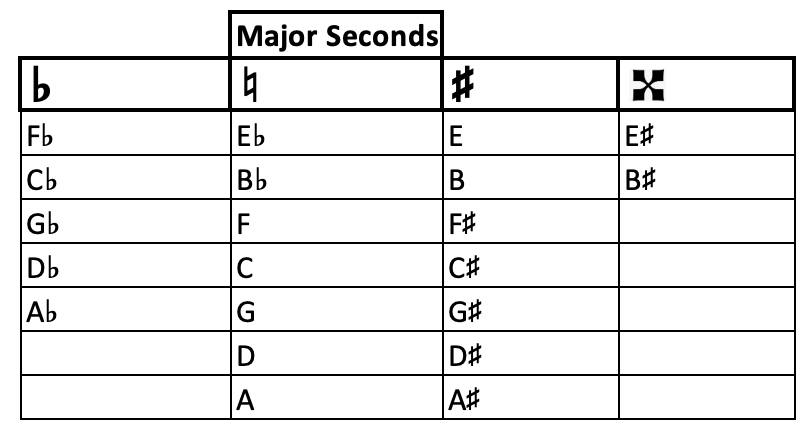
\includegraphics[width=0.5\textwidth]{images/maj_seconds}
\caption{Accidental of Major Second from Tonic per Key}
\label{maj_seconds}
\end{figure}

This allows us to ascertain that in any key, the note that is a major second above the tonic has the same accidental as the tonic, except for keys that have the note name E and B. (Namely, these keys are E and B major or minor, E\musFlat\; and B\musFlat\; major or minor, and E\musSharp\; and B\musSharp\; major or minor). In these  cases, the accidental is ``lifted" once  (i.e. \musFlat\; becomes \musNatural, \musNatural\;  becomes \musSharp, and \musSharp\; becomes \musDoubleSharp). This is where the ADT \verb.Accidental.'s derivation of \verb.Enum. comes in. In order to lift or lower an accidental, we can simply apply \verb.succ. or \verb.pred.. Thus, if the note name of the scale key is E or B, we apply \verb.succ. to the accidental in the key name (i.e. the accidental of the tonic) to get the accidental of the note a major second above the tonic. 

We can proceed in a similar fashion for all other imperfect intervals. In the case of thirds, it turns out that the pattern emerges for minor thirds, rather than major thirds.
\newpage
\begin{figure}[h!]
\centering
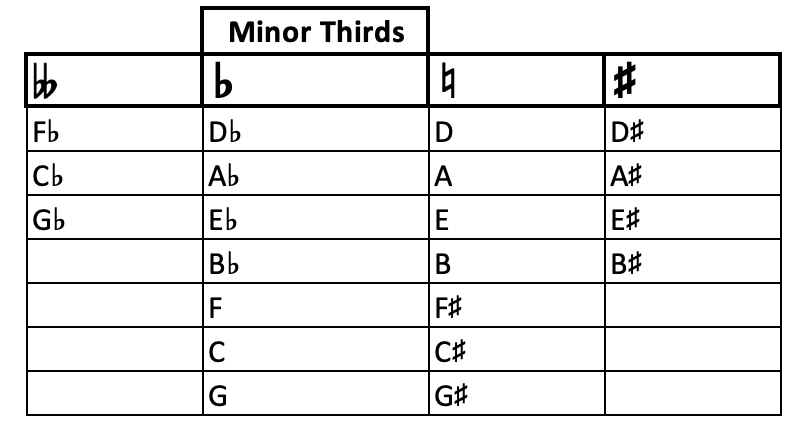
\includegraphics[width=0.5\textwidth]{images/min_thirds}
\caption{Accidental of Minor Third from Tonic per Key}
\label{min_thirds}
\end{figure}

We see that for any key, the note that is a minor third above the tonic has the same accidental as the tonic, except for keys that have the note name F,  C, or G. In these  cases, the accidental is ``lowered" once  (i.e. \musFlat\; becomes \musDoubleFlat, \musNatural\; becomes \musFlat, and \musSharp\; becomes \musFlat). Just like with major seconds, now, if the note name of the key is F, C, or G, we apply \verb.pred. to the accidental in the key name (i.e. the accidental of the tonic) to get the accidental of the note a minor third above the tonic.

Subsequently, the case of sixths, it turns out that the pattern emerges for major sixths, rather than minor thirds.

\begin{figure}[h!]
\centering
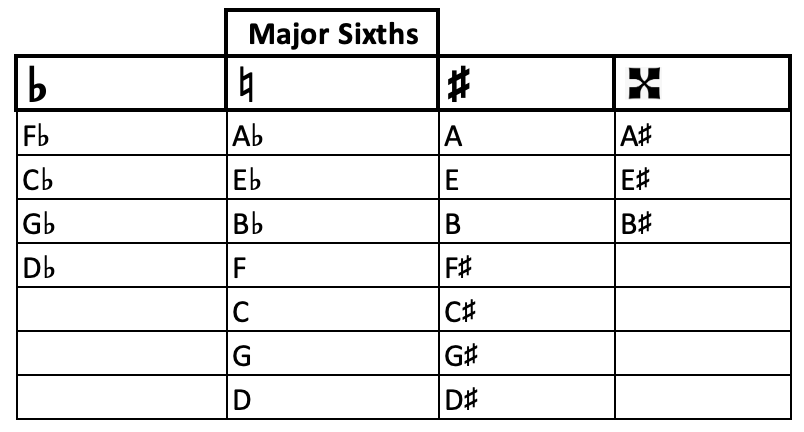
\includegraphics[width=0.5\textwidth]{images/maj_sixths}
\caption{Accidental of Major Sixth from Tonic per Key}
\label{maj_sixths}
\end{figure}

We see that for any key, the note that is a major sixth above the tonic has the same accidental as the tonic, except for keys that have the note name A, E, or B. In these  cases, the accidental is ``lifted" once, like with major seconds. Thus, if the note name of the scale key is A, E, or B, we apply \verb.succ. to the accidental in the key name (i.e. the accidental of the tonic) to get the accidental of the note a major sixth above the tonic.

Finally, the case of sevenths, it turns out that the pattern emerges for minor sevenths, rather than major sevenths.
\newpage

\begin{figure}[h!]
\centering
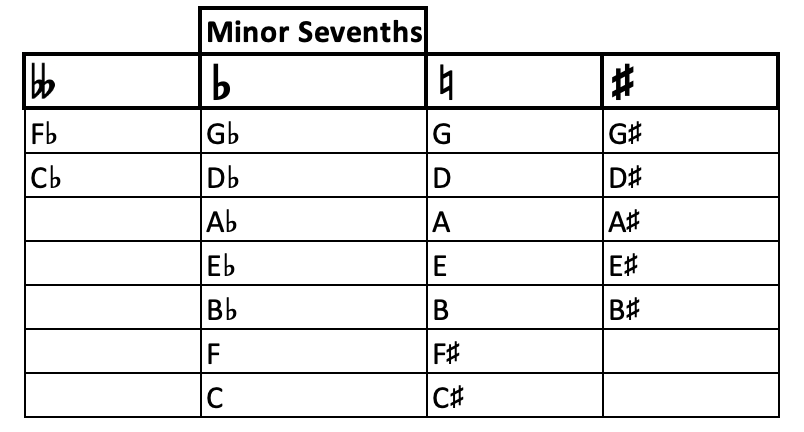
\includegraphics[width=0.5\textwidth]{images/min_sevenths}
\caption{Accidental of Minor Seventh from Tonic per Key}
\label{min_sevenths}
\end{figure}

We see that for any key, the note that is a minor seventh above the tonic has the same accidental as the tonic, except for keys that have the note name F or C. In these  cases, the accidental is ``lowered" once, like with minor thirds. Thus, if the note name of the scale key is F or C, we apply \verb.pred. to the accidental in the key name (i.e. the accidental of the tonic) to get the accidental of the note a minor seventh above the tonic.

We finally consider the perfect intervals: fourths and fifths. By thinking about these intervals for a moment, it becomes clear that perfect intervals always have the same accidental as their tonic, except in those rare cases when we get a tritone. There is only one case that this occurs for each of these intervals: for perfect fourths, keys with F in the key name, and for perfect fifths, keys with B in the note name. The logic for this can be seen by visualizing a piano. B is a tritone above F because B is only a half step (rather than a whole step) below C, and F is a tritone above B because F is only a half step (rather than a whole step) above E.

%-- Map numStepsFromTonic ([notes that are special cases for this interval], 
%                        -- function to alter accidental for special case notes, 
%                        -- quality that the computed accidentals are valid for).
                        
All of these conclusions allow us to summarize our findings in the following map (defined \href{https://github.com/ilanashapiro/MusAssist/blob/main/app/IRConversion.hs}{here}):
\begin{verbatim}
globalStepsFromTonicToAccInfoMap :: Map Int ([MusAST.NoteName],
                                    MusAST.Accidental -> MusAST.Accidental, 
                                    Maybe MusAST.Quality)
globalStepsFromTonicToAccInfoMap = Map.fromList
    [(0, ([], (succ . pred), Nothing)),                            -- root
     (1, (drop 5 globalOrderOfSharps, succ, Nothing)),             -- seconds
     (2, (take 3 globalOrderOfSharps, pred, Just MusAST.Minor)),   -- thirds
     (3, ([MusAST.F], pred, Nothing)),                             -- fourths
     (4, ([MusAST.B], succ, Nothing)),                             -- fifths
     (5, (drop 4 globalOrderOfSharps, succ, Just MusAST.Major)),   -- sixths
     (6, (take 2 globalOrderOfSharps, pred, Just MusAST.Minor))]   -- sevenths
\end{verbatim}

\verb.globalStepsFromTonicToAccInfoMap. maps the interval from tonic (beginning with 0, or the tonic itself) to information about the note at that interval from tonic. In the tuple on the right side of the map, the first element is the list of ``special case" notes from that interval from the tonic (i.e. notes that do not have the same accidental as the tonic). The second element is the function to apply to the tonic accidental in order to get  the correct accidental for these special case notes. The third and final element is the key quality that the accidental pattern is valid for (i.e. major, in the case of sixths, or minor, in the case of thirds and sevenths). Notice that although, based on the pattern discovered in \Cref{maj_seconds}, we would think initially that seconds should only be valid for major keys, this is not the case because both major and minor keys have their supertonic a major second above the tonic. Thus, the valid key quality is \verb.Nothing., since this does not apply here. Similarly, key quality affects neither perfect intervals, nor the tonic itself.

We can thus use \verb.globalStepsFromTonicToAccInfoMap. in \verb.generateToneWithinScale. by querying based on the interval from the tonic. We then adjust the accidental by applying the queried accidental function if the note name is in the special cases list, and then we further adjust based on the key quality the pattern is valid for. For instance, if we are in a major scale and the interval value is 2 (meaning we want a major third), we need to apply \verb.succ. to the accidental from  \verb.globalStepsFromTonicToAccInfoMap.. (Note that we must apply this alteration AFTER we have already applied the queried accidental function if needed). Similarly, if we are in a minor scale and the interval value is 5 (meaning we want a minor sixth), we need to apply \verb.pred. to the accidental from  \verb.globalStepsFromTonicToAccInfoMap. once the queried accidental function has been applied as needed for special octave case notes.

Thus, \verb.generateToneWithinScale. returns the tone within a diatonic scale a specified interval from the tonic, with the option to adjust the octave.

We now return to the function for expanding chord templates. We simply proceed linearly to generate each note in  the chord using \verb.generateToneWithinScale. based on the interval from the tonic. Thirds have an interval of 2 from the tonic, fifths have an interval of 4 from the tonic, and sevenths have an interval of 6 from the tonic.

The scale is set to major for major and augmented chords, and to minor for all other chord qualities (minor, half diminished, diminished). This means that for augmented chords, the chordal fifth will need to be raised half a step (i.e. we need to apply \verb.succ. to the accidental returned in \verb.generateToneWithinScale.), and the chordal seventh will need to be lowered half a step. For diminished chords, both the chordal fifth and seventh will need to be lowered half a step, and for half diminished chords, the chordal fifth will need to get lowered half a step. 

The special octave cases depend on the interval. For instance, for fifths, if the chordal root is F, G, A, or B, the chordal fifth's octave number is one above the root, since octave numbers change on C. We can use the convenient function \verb.enumFromTo. from our custom instance of the \verb.Enum. class for the ADT \verb.NoteName., and we get that the special octave cases for fifths are \verb!(enumFromTo MusAST.F MusAST.B)!, and the octave function to get applied in \verb.generateToneWithinScale. for these cases is \verb.succ.. The same logic applies to all other intervals, by simply working out which chordal roots have the specified interval above them in a different octave. This allows us to make all chords initially in root position. The octave function for \verb.generateToneWithinScale. is always \verb.succ. in chord template expansion (i.e. all special octaves cases in any chord template will have the associated function \verb.succ.), but as we will see later in the expansion of other templates, this is not always the case. 

The final consideration to handle in chord template expansions are inversions. If the chord type is a triad, the chord template expansion stops after generating the notes for the triad. Otherwise, it continues on to generate the chordal seventh. In either case, inversions are handled similarly. Recall that the chord (whether triad or seventh) starts out in root position. Let $n$ be the inversion value (0 for root, 1 for first inversion, 2 for second,  and 3 or third). By incrementing the octaves of the first $n$ tones of the chord in root position, we get the correct inversion. 

At this point,  we have all the information we need for chord template expansion. The computed and adjusted note name, accidental, and octave of for each tone in the chord are zipped together to create a list of  tones, and this is passed into the data constructor \verb.Chord. from the ADT \verb.Expr.. The given duration  for the chord template is passed in as the second parameter for \verb.Chord., and we are done.

%--------------------------------------------------------------------------------------------------------------------------------------------------------

\subsection{Cadences}
Recall that a cadence template contains information about its cadence type, start tone, quality, and duration, where duration is the length of each note, and start tone and quality together determine the local key of the cadence. It will get expanded to the list of chords that it describes.

Expansion of cadences begins a validity check: that the quality of the cadence is either major or minor. After this, the chords of the cadences are generated.

To do this, a helper function called \verb.generateTriadWithinScale. was created. This function, given the tonic tone and quality (either major or minor), will generate the triad within that diatonic scale given the desired inversion and interval from the tonic (must be between 0 and 6, i.e. within one octave of the tonic) and inversion. Given the tonic quality (i.e. the quality of the scale), \verb.generateTriadWithinScale. first determines the quality of the desired chord. From music theory, it is known that that major keys contain the following chords: I-ii-iii-IV-V-vi-vii$^\text{o}$, and minor keys contain the following chords: i-ii$^\text{o}$-III-iv-v-VI-VII. Thus, depending on whether the tonic quality is major or minor, the quality of the triad is computed based on this information.

After this, \verb.generateToneWithinScale. is called to  generate the root of the chord. Following this, a chord template for the triad is created, and passed into \verb.expandIntermediateExpr. to get expanded into a \verb.Chord. containing the list of tones and durations. The result of this is the desired triad.

Returning to cadence template expansion, \verb.generateTriadWithinScale. is used to create each triad in  the cadence. Notably, none of the cadences in MusAssist utilize seventh chords. 
\\\verb.generateTriadWithinScale. is thus called to generate the chords for the given cadence type based on MusAssist's cadence representations from \Cref{table:cadences}. 

A notable edge case that occurred was when creating the V$^{6 \atop 4}$ chord for deceptive cadences. In order for the cadence to render appropriately, the root of the V$^{6 \atop 4}$ needs to be an octave number $below$ the tonic of the scale. Hence, the special octave cases are \verb!(enumFromTo MusAST.C MusAST.E)! (i.e. C,D, and E, the keys whose  fifth scale degree would normally be the $same$ octave number as the tonic), and the octave function for these cases is  \verb.pred.

Other edge cases included making sure that all V chords were major when calling \\\verb.generateTriadWithinScale., no matter the local key quality, since in a cadence, the five chord is always major. Similarly, we want the diminished seventh triad vii$^\text{o}$ in the imperfect authentic cadence no matter the local key quality (since we raise the leading tone in minor keys when moving towards the tonic). This means that  we also to pass major as the quality parameter to \verb.generateTriadWithinScale. here, in order for this chord to be built off the major seven scale degree.

After creating all the chords for the cadence  type with  \verb.generateTriadWithinScale., the chords are simply returned as a list.

%--------------------------------------------------------------------------------------------------------------------------------------------------------
\subsection{Harmonic Sequences}
Harmonic sequences were the most complex template to expand. In order to generate a harmonic sequence, three items need to be determined: (1) the interval of the next chord relative to the previous, (2) the inversion of each chord, and (3) the octave number of each chord.

The following diagrams demonstrate the interval pattern for each sequence based on the chord index. All sequences use zero-indexing.  (Refer to \Cref{sec:harmseq} for the first description of these harmonic progressions).

\begin{figure}[h!]
\centering
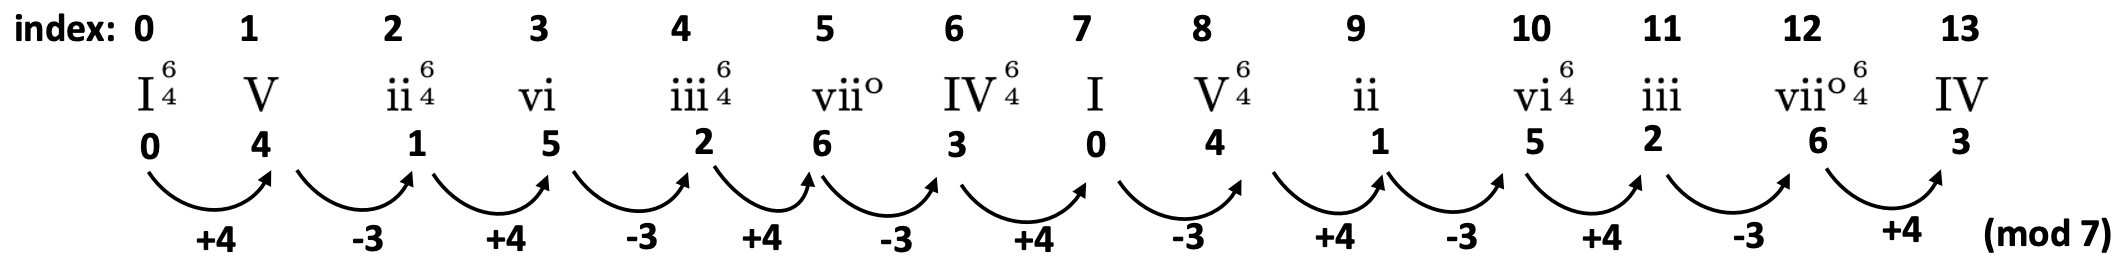
\includegraphics[width=\textwidth]{images/asc_fifths_intervals}
  \caption{Ascending Fifths Interval Analysis}
\end{figure}

\begin{figure}[h!]
\centering
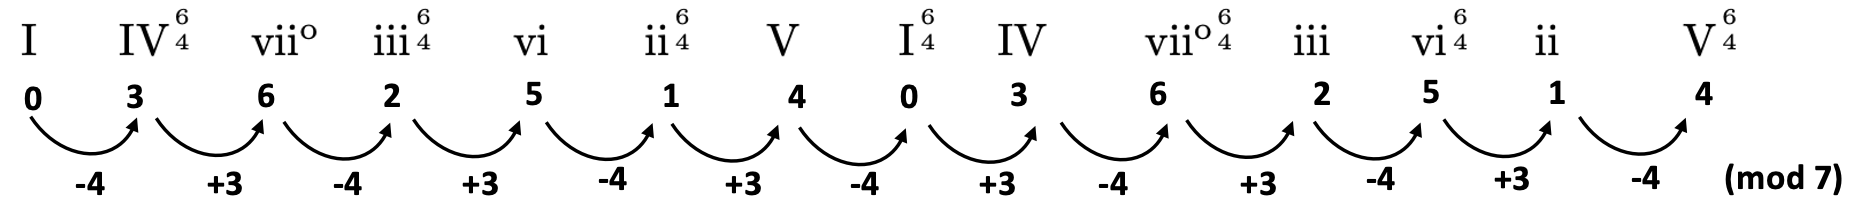
\includegraphics[width=\textwidth]{images/desc_fifths_intervals}
  \caption{Descending Fifths Interval Analysis}
\end{figure}

\begin{figure}[h!]
\centering
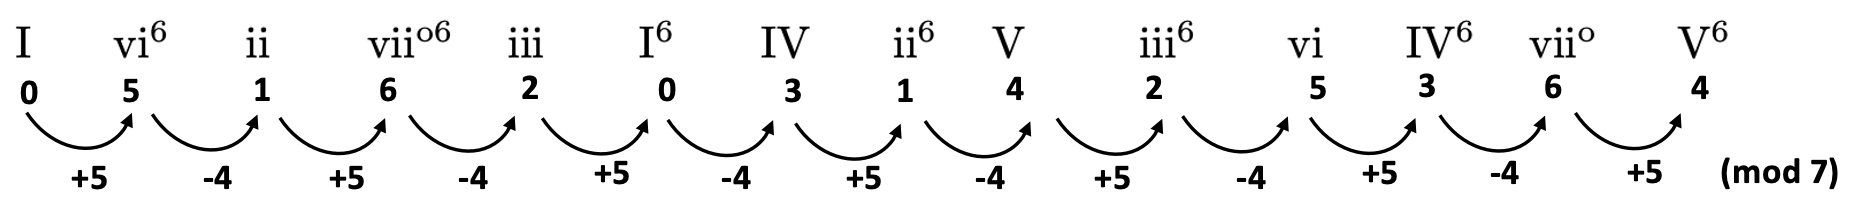
\includegraphics[width=\textwidth]{images/asc_56_intervals}
  \caption{Ascending 5-6 Interval Analysis}
\end{figure}

\begin{figure}[h!]
\centering
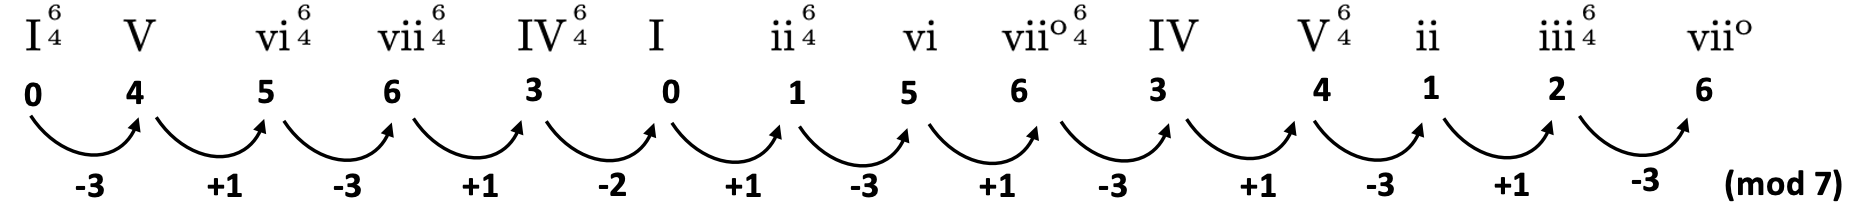
\includegraphics[width=\textwidth]{images/desc_56_intervals}
  \caption{Descending 5-6 Interval Analysis}
\end{figure}

In each figure, the top row is the chord index, the second row is the chord progression, the third row is the interval of the chord from the tonic, and the bottom row is the interval of each chord from the previous (modulo 7). A clear pattern for both chord inversions and interval changes emerges for each sequence based on the index. Also, recall from Figures \ref{fig:ascfifths} -- \ref{fig:desc56} that all descending sequences are written in a descending direction, and ascending sequences are written in an ascending direction. Thus, when descending sequences repeat, their octave number decrements, and when ascending sequences repeat, their octave number increments. We can thus write Haskell code to create the following tuples of (first chord in sequence, octave number change when the sequence repeats, interval from previous chord when at an even index, interval from previous chord when at an odd index, even index chord inversion, odd index chord inversion) for each sequence:

% -- the "index interval changes" tell you how to get to the next chord in the seq, from the current chord, via the interval separating them
\begin{verbatim}
(tonicTriad, octIncVal, evenIndexIntervalChange, oddIndexIntervalChange, evenIndexInv, 
 oddIndexInv) = case harmSeqType of 
    MusAST.AscFifths  -> (tonicSecondInvTriad, 1, 4, -3, MusAST.Root, MusAST.Second)
    MusAST.DescFifths -> (tonicRootTriad, -1, -4, 3, MusAST.Second, MusAST.Root)
    MusAST.Asc56      -> (tonicRootTriad, 1, 5, -4, MusAST.First, MusAST.Root)
    MusAST.Desc56     -> (tonicSecondInvTriad, -2, -3, 1, MusAST.Root, MusAST.Second)
\end{verbatim}

The next step is to determine the octave number of each chord. Recall that the octave number of a chord in the sequence is given by the octave number of the chordal root (no matter the inversion). Also, the octave number of each chord depends only on the note name, not the accidental (since all an accidental does is alter the same note in the staff). By going through each sequence for each of the seven possible notes in a key name (i.e. CDEFFGAB), we determine the octave number of each chord relative to the octave of the first chord in the sequence. To do this, all chords were converted to root position for the sake of the analysis. For instance, consider \Cref{fig:desc56-example}. 

\begin{figure}[h!]
\centering
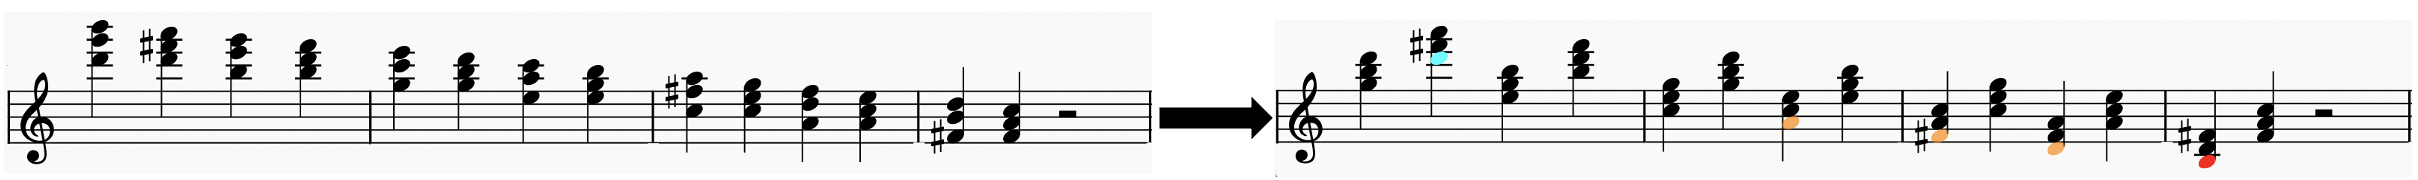
\includegraphics[width=1.1\textwidth]{images/desc56-example}
  \caption{Descending 5-6 Octaves Example}
  \label{fig:desc56-example}
\end{figure}

The chordal roots in blue are an octave number above the first chord in the sequence,  the chordal roots in yellow are an octave number below, and the chordal  root in red is two octave numbers below.

By doing this analysis for each key name, per sequence, the following information was gathered for each sequence, revealing patterns based on the chord indices in the sequences.

We begin by considering ascending fifths. For each possible key name (i.e. each possible note name), \Cref{fig:asc_fifths_octave_grid} shows the function that relates the octave number of the chord at that index in the sequence to the octave number of the first chord in the sequence (assuming zero-indexing of chords). For instance, given an ascending fifths sequence with C in the key name (i.e., C\musFlat, C\musNatural, or C\musSharp \; major or minor), then the chords at indices 7,9,11, and 13 in the sequence (using zero-indexing) will be an octave number above the first chord in the sequence.

\begin{figure}[h!]
\centering
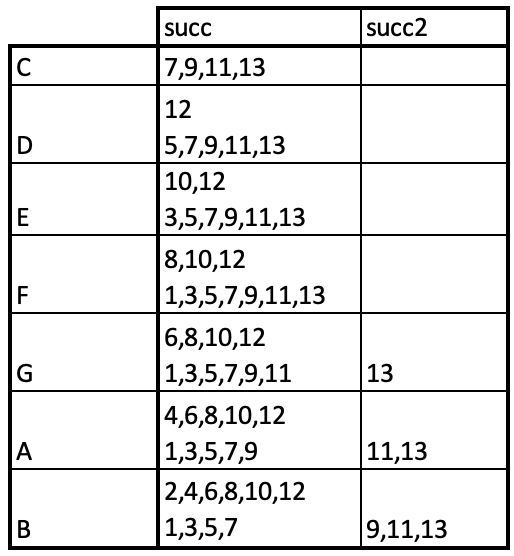
\includegraphics[width=0.3\textwidth]{images/asc_fifths_octave_grid}
  \caption{Ascending Fifths Octave Table}
  \label{fig:asc_fifths_octave_grid}
\end{figure}
\newpage
 \Cref{fig:asc_fifths_octave_grid} was then transposed and reorganized in  \Cref{fig:asc_fifths_octave_analysis} to relate indices to key names. Note that \verb.succ2. is shorthand for \verb!succ . succ!

\begin{figure}[h!]
\centering
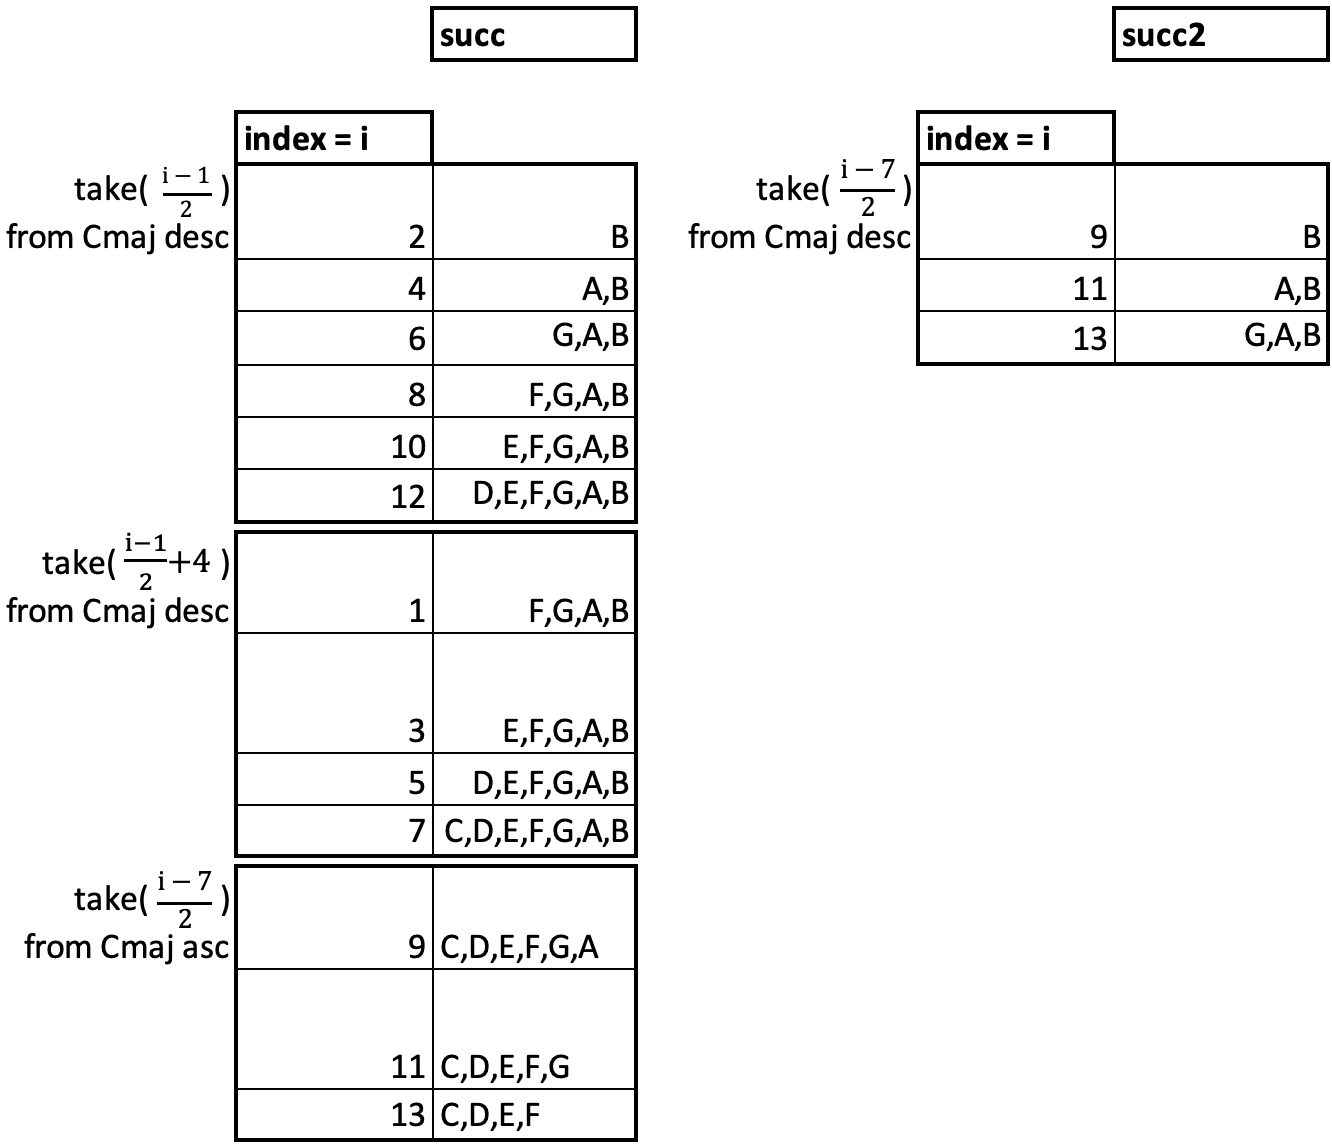
\includegraphics[width=0.7\textwidth]{images/asc_fifths_octave_analysis}
  \caption{Ascending Fifths Octave Analysis}
  \label{fig:asc_fifths_octave_analysis}
\end{figure}
\newpage

As demonstrated in the figure, this allows us to create rules based on chord indices in the sequence. For each function (here, \verb.succ. and \verb.succ2.) that relates chord octave numbers to the octave number of the first chord the sequence, the indices were ``chunked" into groups that can each be described by a single function, whose input is the index and whose output is the key name. For instance, all even-indexed chords in an ascending fifths sequence may need to have their octave  number increased relative to the first chord, depending on the key name. For any such even index $i$, we can determine which sequence key names must have the octave number of their $i^{th}$ chord increased relative to the first chord by taking the first $\frac{i-1}{2}$ key names (i.e. note names) from the C major descending scale (B,A,G,F,E,D,C). 

This allows us to write the following code to determine the octave number of each chord in the ascending fifths sequence, relative to the first chord. Given the chord index in the sequence, we generate a pair relating the special octave cases (i.e. key names) with their associated alteration functions so that we correctly alter the octave number of the first chord to obtain the octave number of the chord at the desired index. For instance if we were at index 1 in a sequence, we would get ([F,G,A,B], \verb.succ.), since sequences in any of these keys have their index 1 chord an octave number above the first chord.

\begin{verbatim}
    if even nextIndexInSeq 
        then (take (nextIndexInSeq `div` 2) cMajScaleNotesDesc, succ)
    else if nextIndexInSeq <= 7
            then (take ((nextIndexInSeq - 1) `div` 2 + 4) cMajScaleNotesDesc, succ)
    else let (succ2Cases, succCases) = splitAt ((nextIndexInSeq - 7) `div` 2) cMajScaleNotesDesc
            in if tonicNoteName `elem` succ2Cases 
                    then (succ2Cases, succ2) 
                else (succCases, succ)
\end{verbatim}

Unfortunately, however, the relations from chord index to special octave cases are not always functions, unless we restrict their use cases. Let $f(i) = \frac{i-7}{2}$ Returning to \Cref{fig:asc_fifths_octave_analysis}, we see that, for instance, $f(9) =$ \{C,D,E,F,G,A\} for \verb.succ., but also $f(9) =$ \{B\} for \verb.succ2.. A similar issue occurs for $f(11)$ and $f(13)$. In order to make $f$ a function, we need to determine which result set it maps to (i.e. to the set of key names for \verb.succ., or the set of key names for \verb.succ2.). 

For $i \in \{9,11,13\}$, let $f(i)$ be the resulting set of key names for \verb.succ., and let $f(i)$' be the resulting set of key names for \verb.succ2.. Fortunately, we note that $f(i) \cap f(i)' = \emptyset$, and $f(i) \cup f(i)' = $ C major scale (i.e. \{C,D,E,F,G,A,B\}). In other words, the result sets are cleanly divided by splitting the C major descending scale (i.e. \{B,A,G,F,E,D,C\}) at the $\frac{i-7}{2}^{th}$ note (i.e. the first $\frac{i-7}{2}$ notes of this scale will map to the result set for  \verb.succ2., and the remaining notes will map to the result set for \verb.succ). This is exemplified in the following line from the ascending fifths octaves code above:

\verb.let (succ2Cases, succCases) = splitAt ((nextIndexInSeq - 7) `div` 2) cMajScaleNotesDesc.

We have thus split the result sets into \verb.(succ2Cases, succCases). In order to determine which result set we want to $f$ to map to, we simply see which set contains  the  tonic note name (i.e. the key note name), we we call $n$. Since we just concluded that $f$  covers the entire C major scale (and thus all key names) over both its possible result sets, we know that we always have  $n \in f(i)$. Thus, either $n \in$ \verb.succ2Cases., or $n \in$ \verb.succCases.. If the former is true, then, as seen in the above code, our result is \verb.(succ2Cases, succ2).. Otherwise, we simply have \verb.(succCases, succ). 

The special octave key names and their respective associated octave alteration functions are thus determined for the ascending fifths sequence. An identical analysis can be applied to the remaining sequences to determine their octave information.

For the descending fifths sequence, Figures \ref{fig:desc_fifths_octave_grid} and \ref{fig:desc_fifths_octave_analysis} similarly describe the relationship between chord index and octave number relative to the first chord in the sequence. Notice here that rather than \verb.succ. and \verb.succ2., we have \verb.pred. and \verb.pred2. (shorthand for \verb!pred . pred!), indicating that octave numbers are lowered by one or two from the first chord, depending on the chord index.

\begin{figure}[h!]
\centering
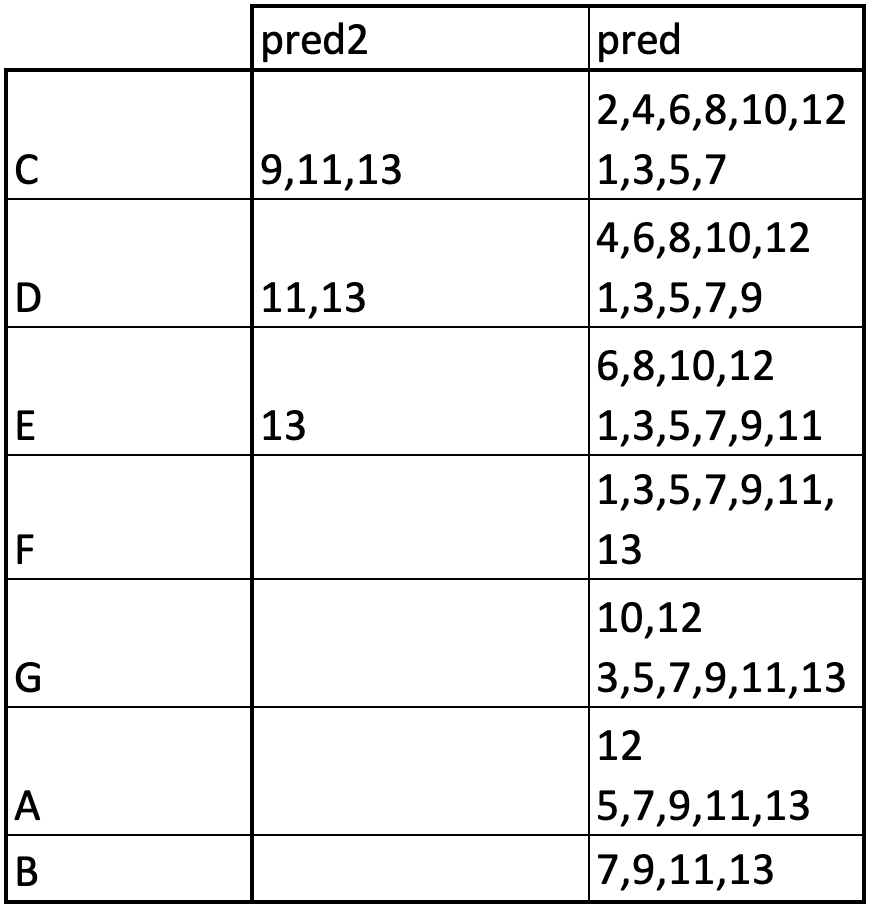
\includegraphics[width=0.4\textwidth]{images/desc_fifths_octave_grid}
  \caption{Descending Fifths Octave Table}
  \label{fig:desc_fifths_octave_grid}
\end{figure}

\begin{figure}[h!]
\centering
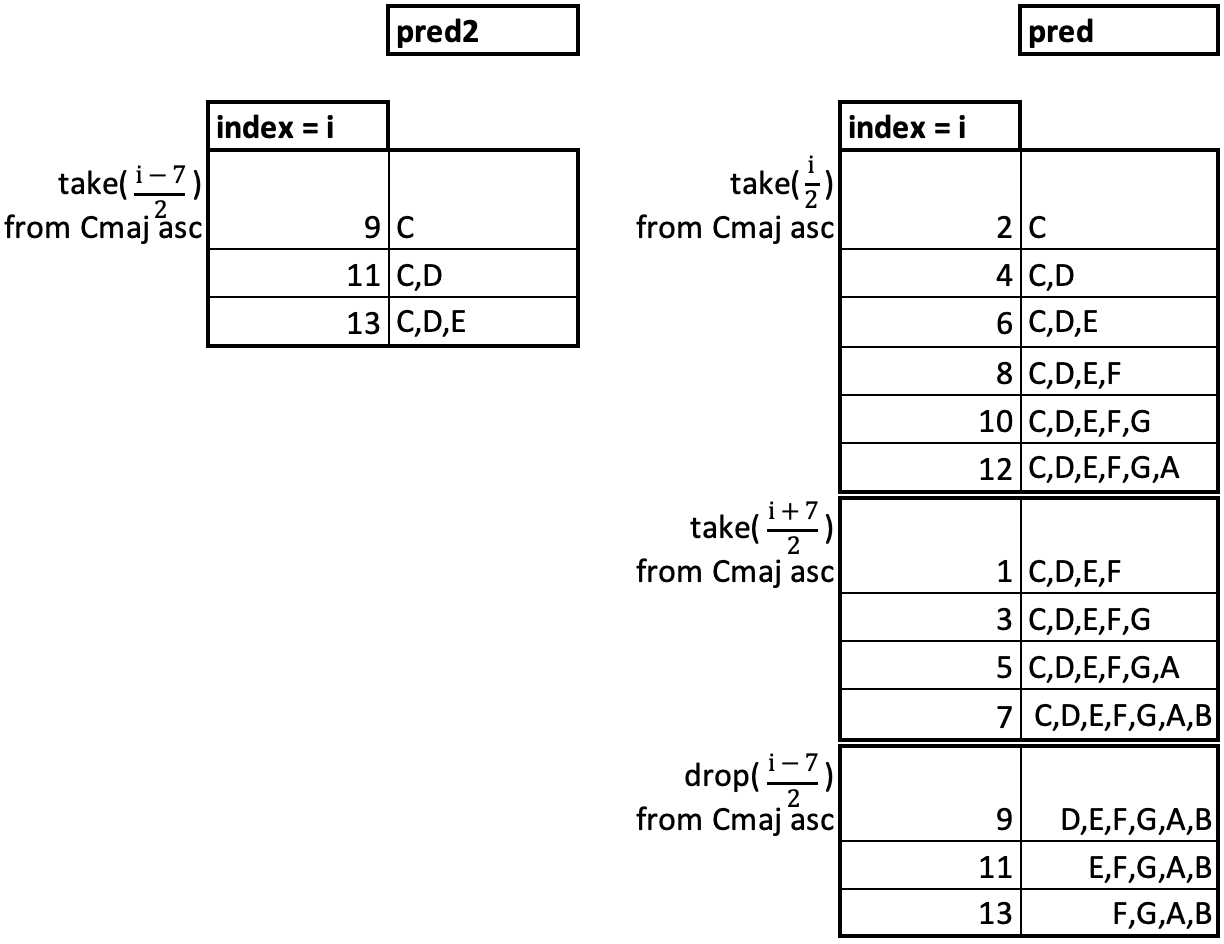
\includegraphics[width=0.7\textwidth]{images/desc_fifths_octave_analysis}
  \caption{Descending Fifths Octave Analysis}
  \label{fig:desc_fifths_octave_analysis}
\end{figure}
\newpage
Like the ascending fifths sequence, here we can similarly use the conclusions from Figures \ref{fig:desc_fifths_octave_grid} and \ref{fig:desc_fifths_octave_analysis} to write the following code to determine the special octave cases (i.e. key names) and their respective associated alteration functions for the descending fifths sequence.

\begin{verbatim}
    if even nextIndexInSeq 
        then (take (nextIndexInSeq `div` 2) cMajScaleNotesAsc, pred)
    else if nextIndexInSeq <= 5
        then (take ((nextIndexInSeq + 7) `div` 2) cMajScaleNotesAsc, pred)
    else 
        let (pred2Cases, predCases) = splitAt ((nextIndexInSeq - 7) `div` 2) cMajScaleNotesAsc
        in if tonicNoteName `elem` pred2Cases 
                then (pred2Cases, pred2) 
            else (predCases, pred)
\end{verbatim}

Notice that here we also have to split the result sets for $f(i) = \frac{i-7}{2}$ when $i \in \{9,11,13\}$. Just like before, we have $f(i) \cap f(i)' = \emptyset$, and $f(i) \cup f(i)' =$ C major scale. We can thus definitively split  the relation into two cases to make it a function with the following line:

\verb.let (pred2Cases, predCases) = splitAt ((nextIndexInSeq - 7) `div` 2) cMajScaleNotesAsc.

and depending which result set the tonic note name is in, we know to return that result set and its associated octave alteration function (i.e. either \verb.(pred2Cases, pred2). or \verb.(predCases, pred).).

We continue this analysis for the ascending 5-6 sequence in Figures \ref{fig:asc_56_octave_grid} and \ref{fig:asc_56_octave_analysis}.

\begin{figure}[h!]
\centering
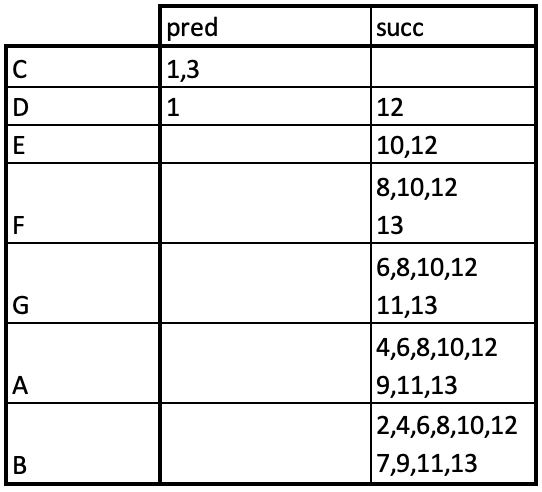
\includegraphics[width=0.4\textwidth]{images/asc56_octave_grid}
  \caption{Ascending 5-6 Octave Table}
  \label{fig:asc_56_octave_grid}
\end{figure}

\begin{figure}[h!]
\centering
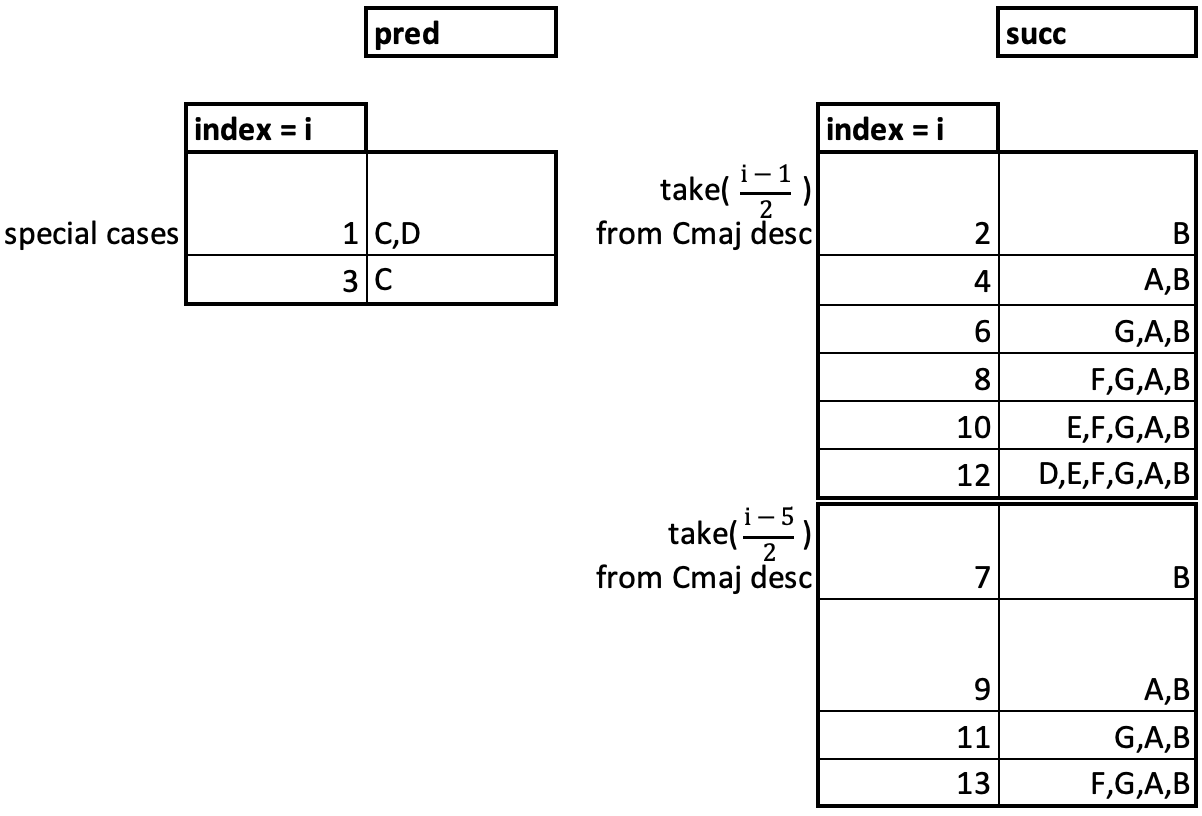
\includegraphics[width=0.7\textwidth]{images/asc56_octave_analysis}
  \caption{Ascending 5-6 Octave Analysis}
  \label{fig:asc_56_octave_analysis}
\end{figure}
\newpage

From these tables, we come up with the following code:

\begin{verbatim}
    if even nextIndexInSeq 
        then (take (nextIndexInSeq `div` 2) cMajScaleNotesDesc, succ)
    else if nextIndexInSeq >= 7  
        then (take ((nextIndexInSeq - 5) `div` 2) cMajScaleNotesDesc, succ)
    else if nextIndexInSeq <= 3 
        then (take (if nextIndexInSeq == 1 then 2 else 1) cMajScaleNotesAsc, pred)
    else ([], const nextTonicOctave)  
\end{verbatim}

\noindent Note that here, we do not need to split up the  result sets for any of the relations,  as they are all functions to begin with (i.e. each index maps to a single result set). However, we do have one new case: the final line, \verb.([], const nextTonicOctave)., in which no special octave cases exist for that index. Specifically, in this case, the index 5 chord in the ascending 5-6 sequence (i.e. the sixth chord due to zero-indexing) is simply the first chord again, albeit in a different inversion, and thus always has the same octave number as the first chord, no matter the key name. \verb.const nextTonicOctave. is therefore a placeholder for this case when there is  no special octave function to be applied.
         
Finally, we apply the analysis one more time for the descending 5-6 sequence, as see in Figures \ref{fig:desc_56_octave_grid} and  \ref{fig:desc_56_octave_analysis}.

\begin{figure}[h!]
\centering
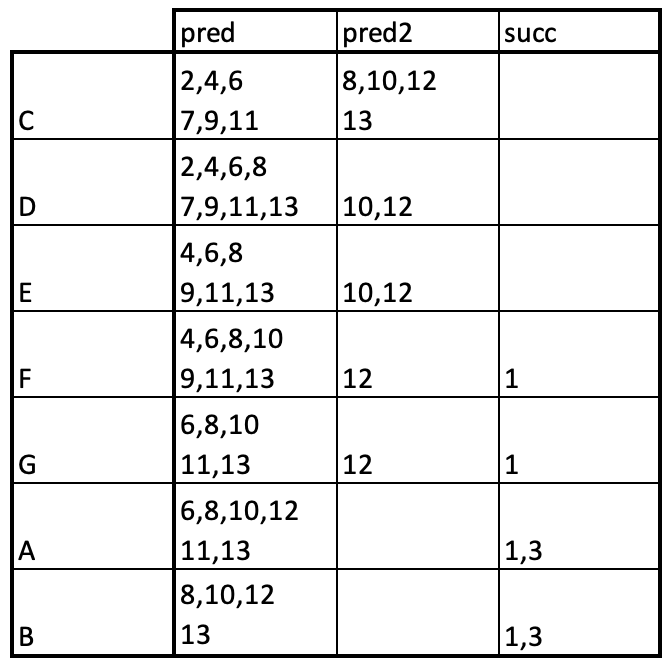
\includegraphics[width=0.4\textwidth]{images/desc56_octave_grid}
  \caption{Descending 5-6 Octave Table}
  \label{fig:desc_56_octave_grid}
\end{figure}

\begin{figure}[h!]
\centering
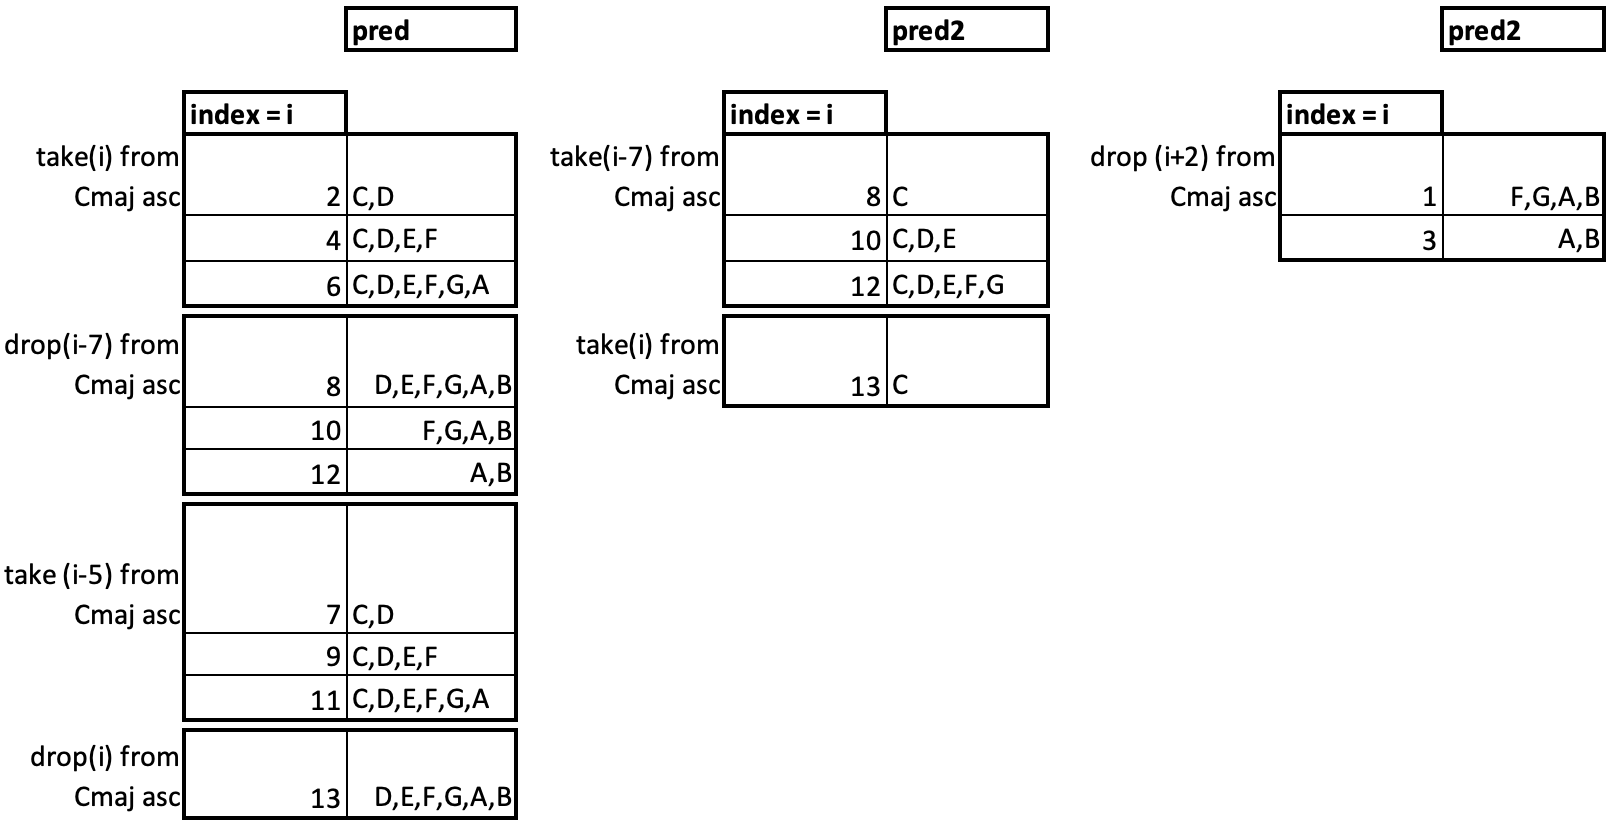
\includegraphics[width=\textwidth]{images/desc56_octave_analysis}
  \caption{Descending 5-6 Octave Analysis}
  \label{fig:desc_56_octave_analysis}
\end{figure}
\newpage

Note that for the first time, we have three octave function cases: \verb.pred., \verb.pred2., and \verb.succ.. This is reflected in the following Haskell implementation.

\begin{verbatim}
    if even nextIndexInSeq 
        then if nextIndexInSeq <= 6 then (take nextIndexInSeq cMajScaleNotesAsc, pred)
                else let (pred2Cases, predCases) = splitAt (nextIndexInSeq - 7) cMajScaleNotesAsc
                    in if tonicNoteName `elem` pred2Cases 
                           then (pred2Cases, pred2) 
                        else (predCases, pred)
    else if nextIndexInSeq == 13
            then let (pred2Cases, predCases) = splitAt 1 cMajScaleNotesAsc
                in if tonicNoteName `elem` pred2Cases 
                        then (pred2Cases, pred2)
                    else (predCases, pred)
    else if nextIndexInSeq >= 7
        then (take (nextIndexInSeq - 5) cMajScaleNotesAsc, pred)
    else if nextIndexInSeq <= 3
        then (drop (nextIndexInSeq + 2) cMajScaleNotesAsc, succ)
    else ([], const nextTonicOctave) 
\end{verbatim}

Here, we must split two relations, $f_1(i) = i-7$, where $i \in \{8,10,12\}$, and $f_2(i) = 1$, where $i =13$, into two respective result sets in order to make them functions. Just like before, we have $f_1(i) \cap f_1(i)' = f_2(i) \cap f_2(i)' = \emptyset$ for the respective valid values of $i$, as well as $f_1(i) \cup f_1(i)' = f_2(i) \cup f_2(i)' =$ C major scale, for the respective valid values of $i$. We can thus definitively split both relations into two cases to make them each a function, with the following lines taken from the above code:

\noindent \verb.let (pred2Cases, predCases) = splitAt (nextIndexInSeq - 7) cMajScaleNotesAsc. \\(for $i \in \{8,10,12\}$)

\noindent and 

\noindent \verb.let (pred2Cases, predCases) = splitAt 1 cMajScaleNotesAsc. \\(for $i =13$)

Just as before, depending which result set the tonic note name is in, we know to return that result set and its associated octave alteration function (i.e. for both $f_1$ and $f_2$, either \verb.(pred2Cases, pred2). or \verb.(predCases, pred).).

Finally, notice that the \verb.const. function appears once again in the final line of the above code: \verb.([], const nextTonicOctave)..  This again is the situation in which no special octave cases exist for that index. Specifically, just like the ascending 5-6 sequence, the index 5 chord in the descending 5-6 sequence (i.e. the sixth chord due to zero-indexing) is simply the first chord again, albeit in a different inversion, and thus always has the same octave number as the first chord, no matter the key name.

We have thus determined how to find the interval and inversion of a chord in the sequence from the previous chord, and how to find the octave number of a chord in the sequence. Importantly, the interval analysis holds for any representation of these harmonic sequences, as this is what defines the sequence. However, the inversion and octave analysis holds only for MusAssist's chosen representation of the sequences, as a different inversion pattern would deeply alter both of these analyses.

We are now ready to generate the sequences. A generic sequence-generator helper function called \verb.generateSeq n. was written that, given $n$ (the length, or number of chords) in the sequence, generates the sequence. \verb.generateSeq n. determines the next index  in the sequence (resetting to zero each  time the sequence repeats after 14 chords), either  increments or decrements the tonic octave number after each cycle, determines the note name of the next chordal root based on the interval rule from the previous chord for that sequence, and determines the inversion based on the index. The special octave cases and associated octave functions are passed in based on the previously discussed analysis. \verb.generateSeq n. now has enough information to call  \verb.generateTriadWithinScale. to generate the desired chord for that index in the sequence, and then recurses to the next chord in the sequence until $n$ goes to zero. 

%--------------------------------------------------------------------------------------------------------------------------------------------------------
\chapter{Code Generation}
\label{chap:codegen}
We are finally ready to generate MusicXML code from the abstract syntax. In order to do so, we must first comprehend MusicXML's concrete syntax. 

%--------------------------------------------------------------------------------------------------------------------------------------------------------
\section{MusicXML Syntax}
This section gives an overview of MusicXML's syntax as pertains to translations from MusAssist. A full and more detailed reference of MusicXML's syntax can be found \href{https://www.w3.org/2021/06/musicxml40/}{here}.

\noindent Throughout the section, words in all caps (e.g. DURATION) are parameters.

\subsection{Header Code}
\label{sec:xmlheader}
Static MusicXML header code is generated for all MusAssist files that handles encoding, print and midi settings, and layout defaults. The tempo is also set to \musQuarter=80bpm. The header code can be found \href{https://github.com/ilanashapiro/MusAssist/blob/main/app/Compile.hs}{here}. This code was generated by exporting an empty MuseScore file to MusicXML.

However, a critical part of the MusicXML header is left off the static header code until code generation: the program attributes. (This can be found \href{https://github.com/ilanashapiro/MusAssist/blob/main/app/MusicXMLgen.hs}{here}).

\begin{verbatim}
<attributes>
    <divisions>4</divisions>
    <key>
        <fifths>NUM_ACCIDENTALS</fifths>
    </key>
    <time>
        <beats>4</beats>
        <beat-type>4</beat-type>
    </time>
    <clef>
        <sign>G</sign>
        <line>2</line>
    </clef>
</attributes>
\end{verbatim}

The addition of the header attributes was delayed until code generation due to the NUM\_ACCIDENTALS parameter. By default, NUM\_ACCIDENTALS is set to zero, indicating a key signature of C major/A minor. However, if the user's first command is to set the key signature to something else, then the header attributes must be adjusted accordingly. Thus, the helper function \verb.globalHeaderCode fifths. was created, that takes as a parameter the number of sharps or flats. \verb.fifths., which represents NUM\_ACCIDENTALS, is an integer taken from $[-7,7]$. Negative values indicate flats, while positive values indicates sharps.

As for the remainder of the attributes code, the following sets the time signature to common time:
\begin{verbatim}
    <time>
        <beats>4</beats>
        <beat-type>4</beat-type>
    </time>
\end{verbatim}

\noindent and the following sets the clef to treble:
\begin{verbatim}
    <clef>
        <sign>G</sign>
        <line>2</line>
    </clef>
\end{verbatim}

Finally, notice the \verb.<divisions>4</divisions>. element at the top. The \verb.<divisions>. tag is critical to the representation of note durations throughout the MusicXML program. The \verb.<divisions>. value determines the numerical value of the smallest possible duration, which must always be a positive integer. Specifically, the \verb.<divisions>. value determines which division of the quarter note should receive the duration value of one. Since the smallest duration that MusAssist supports is  sixteenth  notes, \verb.<divisions>. is set to four to indicate that one fourth of a quarter note will receive the smallest possible duration of one.

%--------------------------------------------------------------------------------------------------------------------------------------------------------
\subsection{Notes and Chords}
\label{sec:xmlnotes}
A pitched note element in MusicXML has the following form. (The \verb.*. and \verb.+. symbols are not part of the MusicXML code, and indicate optional lines. )

\begin{verbatim}
<note>
    <chord/>+
    <pitch>
        <step>NOTE_NAME</step>
        <alter>ACCIDENTAL</alter>
        <octave>OCTAVE</octave>
    </pitch>
    <duration>DURATION</duration>
    <tie type="start"/>*
    <tie type="stop"/>*
    <voice>1</voice>
    <type>TYPE</type>
    <dot/>+
    <notations>*
        <tied type="start"/>*
        <tied type="stop"/>*
    </notations>*
</note>
\end{verbatim}

\noindent (full details \href{https://www.w3.org/2021/06/musicxml40/musicxml-reference/elements/note/}{here})

The \verb.*. indicate lines that create a start and/or stop tie for the note. If a start or stop tie is used, it must be declared in the \verb.<notations>. element. If the note is not tied either way, the \verb.<notations>. element can be left off completely. The \verb.+. denotes the optional chord and dot tags. The \verb.<chord>. tag is included if the current note is part of a chord with the previous note, and the \verb.<dot>. tag is included when the note has a dotted duration (e.g. dotted quarter note).

NOTE\_NAME is taken from the set \{A,B,C,D,E,F,G\}, and ACCIDENTAL is taken from the set $\{-2,-1,0,1,2\}$. ACCIDENTAL indicates the chromatic alteration of the pitch in the number of semitones. For instance, -2 indicates a double flat, and 1 indicates a single sharp. (MusicXML also supports additional values for ACCIDENTAL, such as 0.5 for microtones, that MusAssist does not support.) OCTAVE is an integer between 0 and 9 inclusive, though MusAssist only supports octaves 1 through 8.

DURATION is a positive integer that indicates the number of division units this note should have. Recall from \Cref{sec:xmlheader} that in a translated MusAssist program, a DURATION value of 1 indicates a sixteenth note. Thus, a quarter note would have a DURATION value of 4, and so on.

TYPE is the graphical type of the note based on its duration (excluding dotted durations). The possible MusAssist durations give that TYPE is taken from the set \{\verb.16th, eighth, quarter, half, whole.\} (``16th" is indeed represented numerically in MusicXML).

Finally, the \verb.<voice>. value is set to 1 for all MusAssist elements, as multiple voicing (the ability to have simultaneous lines occurring in a single measure) is a more advanced notation element that MusAssist does not currently support. 

%--------------------------------------------------------------------------------------------------------------------------------------------------------
\subsection{Rests}
\label{sec:xmlrest}

A rest element in MusicXML has the following form:
\begin{verbatim}
<note>
    <rest/>
    <duration>DURATION</duration>
    <voice>1</voice>
    <type>TYPE</type>
</note>
\end{verbatim}

A rest is a special kind of \verb.<note>. element, with the \verb.<rest/>. tag instead of pitch information. Thus, DURATION and TYPE take on the same values as in \Cref{sec:xmlnotes}. A rest cannot be tied, nor can it be part of a chord.

%--------------------------------------------------------------------------------------------------------------------------------------------------------
\subsection{Measures}
\label{sec:xmlmeasure}
MusicXML measures are denoted by the opening tag \verb.<measure number="NUMBER">. and the closing tag \verb.</measure>, where NUMBER is a positive integer. All code within these tags belongs to that measure.

%--------------------------------------------------------------------------------------------------------------------------------------------------------
\subsection{Key Signatures}
\label{sec:xmlkeysig}
When the  key signature is changed after the beginning of the piece, the following  code is inserted at the beginning of the measure (i.e. directly after the opening \verb.<measure number="NUMBER">. tag):

\begin{verbatim}
<attributes>
    <key>
        <fifths>NUM_ACCIDENTALS</fifths>
    </key>
</attributes>
\end{verbatim}

Like in the header code in \Cref{sec:xmlheader}, NUM\_ACCIDENTALS is an integer taken from $[-7,7]$.

%--------------------------------------------------------------------------------------------------------------------------------------------------------
\section{MusicXML Code Generation}
We are now ready to make the final translation from abstract syntax to MusicXML. The source code can be found \href{https://github.com/ilanashapiro/MusAssist/blob/main/app/MusicXMLgen.hs}{here}.

%--------------------------------------------------------------------------------------------------------------------------------------------------------
\subsection{State}
Throughout the code generation, the state of three items needed to be maintained: (1) the current beat in measure that we are writing to, (2) the current measure number, and (3) the current key signature. In order for these to be globally accessible in the code generation, IORefs were used to represent each:
\begin{verbatim}
type BeatCounter = IORef.IORef Int
type MeasureCounter = IORef.IORef Int
type KeySignature = IORef.IORef (Int, Int)
\end{verbatim}

Here, key signature is represented as a pair of (num sharps, num flats). At least one of (num sharps, num flats) should be zero, and each should be an integer taken from $[-7,7]$. 

\noindent The 3-tuple of the IORefs for beat, measure, and key signature constitute the program state: 

\verb.type State = (BeatCounter, MeasureCounter, KeySignature). 

\noindent\verb.State. is passed around to each code generation function. 

%--------------------------------------------------------------------------------------------------------------------------------------------------------
\subsection{Instructions Translation}

Code generation begins with the function \verb.transInstrs.. Here, we translate the input list of instructions (i.e. the list of the ADT \verb.Instr.) that is the result of the intermediate expansions. After doing so, we pad the final measure with rests if needed. To accomplish the measure padding, we create a helper function called \verb.generateNoteValueRationalDivisions.. (This function will later also be used for tied notes that spill into the next measure).

\verb.generateNoteValueRationalDivisions. uses a bimap (i.e. a map that supports two-way query) called \verb.globalDurationIntBimap. that maps values from the ADT \verb.Duration. to their associated numerical duration values in the MusicXML code. Again, these numerical duration values are based on the value given to the \verb.<divisions>. element in the header. In other words, \verb.Sixteenth. gets mapped to 1, \verb.Eighth. gets mapped to 2, etc. \verb.generateNoteValueRationalDivisions. passes in the numerical duration values from \verb.globalDurationIntBimap. in descending order, from greatest to least, to the helper function \verb.breakUpNoteValRationally. 

 \verb.breakUpNoteValRationally. breaks up the given duration value into ``valid" duration values (i.e. into the numerical values that map to the values  in \verb.globalDurationIntBimap. that are defined in the ADT \verb.Duration.). In order for this to work,  \verb.breakUpNoteValRationally. greedily breaks up the input duration value: it continually attempts to fill the input duration on the current level of recursion with the largest value from the list (i.e. the values from \verb.globalDurationIntBimap.) that is passed in. This is why the values from \verb.globalDurationIntBimap. are ordered from greatest to least before they are passed in. 

\verb.breakUpNoteValRationally. returns this ``rational break-up" of the given duration as a list of (\verb.Duration. ADT value, duration integer value) pairs, ordered either greatest to least (if we are at the beginning of a measure, like in the case of spilled  tied notes), or least to greatest (if we are not at the beginning of the measure, like in the cases of the first part of tied notes, or when we generate measure padding of rests for a partially filled measure). This ordering of rest values follows standard music notation practices. 

The implementation of \verb.breakUpNoteValRationally. is as follows.

\begin{verbatim}
breakUpNoteValRationally :: [Int] -> Int -> Bool -> IO [(MusAST.Duration, Int)]
breakUpNoteValRationally _ 0 _ = return []
breakUpNoteValRationally [] _ _ = return $ error "cannot generate accurate note divisions" 
breakUpNoteValRationally (noteVal:noteVals) remainingTimeInMeasure isFromMeasStart = do
  if noteVal <= remainingTimeInMeasure then do
    noteDuration <- Bimap.lookupR noteVal globalDurationIntBimap 
    remainingPadding <- breakUpNoteValRationally noteVals 
                          (remainingTimeInMeasure - noteVal) isFromMeasStart
    return $ if isFromMeasStart 
                 then (noteDuration, noteVal):remainingPadding 
             else remainingPadding ++ [(noteDuration, noteVal)]
  else breakUpNoteValRationally noteVals remainingTimeInMeasure isFromMeasStart
\end{verbatim}

After the duration is broken up rationally, the helper function \verb.generateRestsFromDivisions. takes in the result list from  \verb.generateNoteValueRationalDivisions. and generates a list of MusicXML code for rests based on the given durations.

%--------------------------------------------------------------------------------------------------------------------------------------------------------
\subsection{Individual Instruction Translation}
Going one level down, \verb.transInstrs. calls \verb.transInstr. to generate MusicXML code for each \verb.Instr. in the instructions list. This means we pattern match to four cases: \verb.KeySignature Int Int., \verb.NewMeasure., \verb.Write [Expr]., and \verb.Assign Label [Expr]. 

As MusicXML code is generated, the current beat and measure number are handled in the function \verb.updateBeat.. Whenever \verb.updateBeat. is called, the current beat IORef is incremented given the note duration parameter passed into the function. If we have reached the end of the measure (i.e. the updated beat count equals the time per measure) then we generate new measure code (see \Cref{sec:xmlmeasure}), increment the IORef for measure number, and reset the current beat IORef to zero. Time per measure is set at 16 for all programs, since the enforced time signature for a MusAssist program is common time, which has 16 sixteenth notes. 

\verb.updateBeat. is called whenever a note or rest is written, and returns new measure code (which is an empty list if we are not starting a new measure). The implementation of \verb.updateBeat. is as follows.

\begin{verbatim}
updateBeat :: NoteDuration -> State -> IO [CodeLine]
updateBeat noteDuration (currBeatCt, measureCt, _) = do
  currentBeatCount <- IORef.readIORef currBeatCt
  let updatedBeatCount = currentBeatCount + noteDuration 
  if updatedBeatCount == globalTimePerMeasure 
    then do
      measureNum           <- IORef.readIORef measureCt
      IORef.writeIORef currBeatCt 0   
      let incMeasNum = measureNum + 1
      IORef.writeIORef measureCt incMeasNum 
      let newMeasureCode = 
          ["\t\t</measure>", "\t\t<measure number=\"" ++ show incMeasNum ++ "\">"]
      return newMeasureCode
    else do
      IORef.writeIORef currBeatCt updatedBeatCount
      return []
\end{verbatim}

Returning to \verb.transInstr., the translation of the instruction \verb.Assign Label [Expr]. does not generate any MusicXML code. 

Like at the end of \verb.transInstrs., the translation of \verb.NewMeasure. calls \verb.generateNoteValueRationalDivisions. and \verb.generateRestsFromDivisions. to pad the rest of the current measure with rests if necessary, and then generates MusicXML code to create a new measure. 

The translation of \verb.Write [Exprs]. simply calls the function \verb.transExpr. (which will be discussed shortly) to unwrap and translate the expressions it contains, and concatenates the results to generate the resulting list of MusicXML codelines.

%--------------------------------------------------------------------------------------------------------------------------------------------------------
\subsubsection{Key Signatures}

The last case for \verb.transInstr., \verb.KeySignature Int Int., is slightly more complicated. After performing an error check that the key signature is valid (i.e. one or both of the arguments to \verb.KeySignature. must be zero, as a key signature cannot have sharps and flats, and the non-zero argument must be an integer taken from $[-7,7]$), the current key signature, beat in the measure, and measure number are read from the IORefs in \verb.State.. If the new key signature is the same as the current one, empty code is returned, and \verb.State. is not updated. Otherwise, we pad the measure with rests if needed using \verb.generateNoteValueRationalDivisions. and \verb.generateRestsFromDivisions. 

Then, we check if this key signature change occurs at the beginning of the first measure, which means this is the user's first instruction. If this is the case, we simply call \verb.globalHeaderCode fifths. from \Cref{sec:xmlheader}. Otherwise, we pad the current measure with rests and generate a new measure using \verb.generateNoteValueRationalDivisions., \verb.generateRestsFromDivisions., and \verb.updateBeat.. Then, finally, we generate MusicXML code for the new key signature (see \Cref{sec:xmlmeasure}), as MusicXML does not support mid-measure key signature changes. 

%--------------------------------------------------------------------------------------------------------------------------------------------------------
\subsection{Expression Translation}

Going another level down, the final recursive function in the code generation is \verb.transExpr., which translates values from the ADT \verb.Expr. to MusicXML. This means we pattern match to four cases: \verb.Rest Duration., \verb.Chord [Tone] Duration., and \verb.LabeledExpr [Expr].. Generating MusicXML code for \verb.LabeledExpr [Expr]. is simple; we simply call \verb.transExpr. recursively for the list of expressions contained in the label. Rests and chords are more complex.

%--------------------------------------------------------------------------------------------------------------------------------------------------------
\subsubsection{Rests}

In the translation of \verb.Rest.s, we  have two cases:
\begin{enumerate}
\item The rest fits in the current measure. Here, we simply generate code for the entire rest (see \Cref{sec:xmlrest}).

\item The rest spills over into the next measure. Here, we break up the rest duration into two pieces (1) what fits in the current measure (the ``initial duration"), and (2) what  spills over (the ``spilled duration"). Then, we break up the initial rest duration rationally,  call \verb.updateBeat. to generate new measure code, and break up the spilled rests rationally. Finally, we call \verb.generateRestsFromDivisions. twice to generate rationally broken-up rest MusicXML code for the initial duration and for the spilled duration. 

\item We return a list with initial rest code, new measure code, and spilled rest code. 
\end{enumerate}

%--------------------------------------------------------------------------------------------------------------------------------------------------------
\subsubsection{Chords}

In the translation of \verb.Chord.s, we first generate code for all the pitches. Recall that if \verb.[Tone]. has one element, then this \verb.Chord. is simply a note. All subsequent \verb.Tone.s in the list will receive a \verb.<chord/>. tag in the MusicXML code (see: \Cref{sec:xmlnotes}). We accomplish this by using the Haskell function \verb.zipWith., and then \verb.concat., for all the tones in the list with their corresponding list indices. In other words, we zip together the tones and the list \verb![0..]!, which contains their indices. An index greater than zero tells us this tone is part of a multi-note chord.

We then have two cases:
\begin{enumerate}
\item The chord fits in the measure. Here, we simply generate code for the entire chord (see: \Cref{sec:xmlnotes}).

\item The chord spills  over into the  next measure. Unlike rests, we now must manually handle ties. Recall that MusicXML requires separate start and stop ties. Thus, we must do the following
\begin{enumerate}
\item Break up the note duration into the initial duration (that fits in the current measure) and spilled duration (that spills into the next measure). 

\item Call \verb.generateNoteValueRationalDivisions. for the initial duration. Take the head of the initial note divisions list, and create a chord from it with start tie only. Then, we call the helper function \verb.generateTiedNotesFromDivisions. on the remaining initial note divisions. \verb.generateTiedNotesFromDivisions. takes in a list of pitches code and a list of (\verb.Duration. ADT value, duration integer value) pairs, and generates chords from these pitches and durations that each have with both start and stop ties.

\item Call \verb.updateBeat. to generate new measure code. 

\item Call \verb.generateNoteValueRationalDivisions. for the spilled duration. Call \verb.init. to take all but the last element of the spilled note divisions, and pass this into \verb.generateTiedNotesFromDivisions. to generate chords with both start and stop ties. Finally, take the last element of the spilled note divisions, and create a chord with stop tie only.
\end{enumerate}

\item Finally, we return a list with the first initial chord code with start tie only, remaining initial chords code with double ties, new measure code,  spilled chords code with double ties, and the final spilled chord code with stop tie only.
\end{enumerate}



At this point, all the MusicXML code has been generated, and we are ready to open the program in MuseScore or other music notation software.

%--------------------------------------------------------------------------------------------------------------------------------------------------------
\chapter{Sample Programs}
The following examples show MusAssist syntax, and the result of opening the compiled MusicXML code in MuseScore.

\begin{verbatim}
SET_KEY Amaj
(D4 whole) (F#4 quarter) (Ab4 quarter) (G#4 eighth) (rest sixteenth)           
// this is a comment
notes1 = (D4 whole) (F#4 quarter) (Ab4 quarter) (G#4 eighth) (rest whole)  
// note without b or # is considered to be natural
chords1 = ([Bbb5, Db5, C5] half) ([C#5, E5] half) (C6 min triad inv:first quarter) 
(F#4 halfdim seventh inv:second eighth)
(D4 whole) (F#4 quarter) (Ab4 quarter) (G##4 eighth) (rest sixteenth)
([Bbb5, Db5, C5] half) ([C#5, E5] half) (C6 min triad inv:first quarter) 
(F#4 halfdim seventh inv:second eighth)
SET_KEY Dmin
NEW_MEASURE
(DescFifths G5 min quarter length:15) (PerfAuthCadence Eb5 min half)
notes1 chords1 (AscFifths G3 min quarter length:5) chords1 
(PerfAuthCadence Eb5 min sixteenth) chords1
\end{verbatim}

\begin{figure}[h!]
\centering
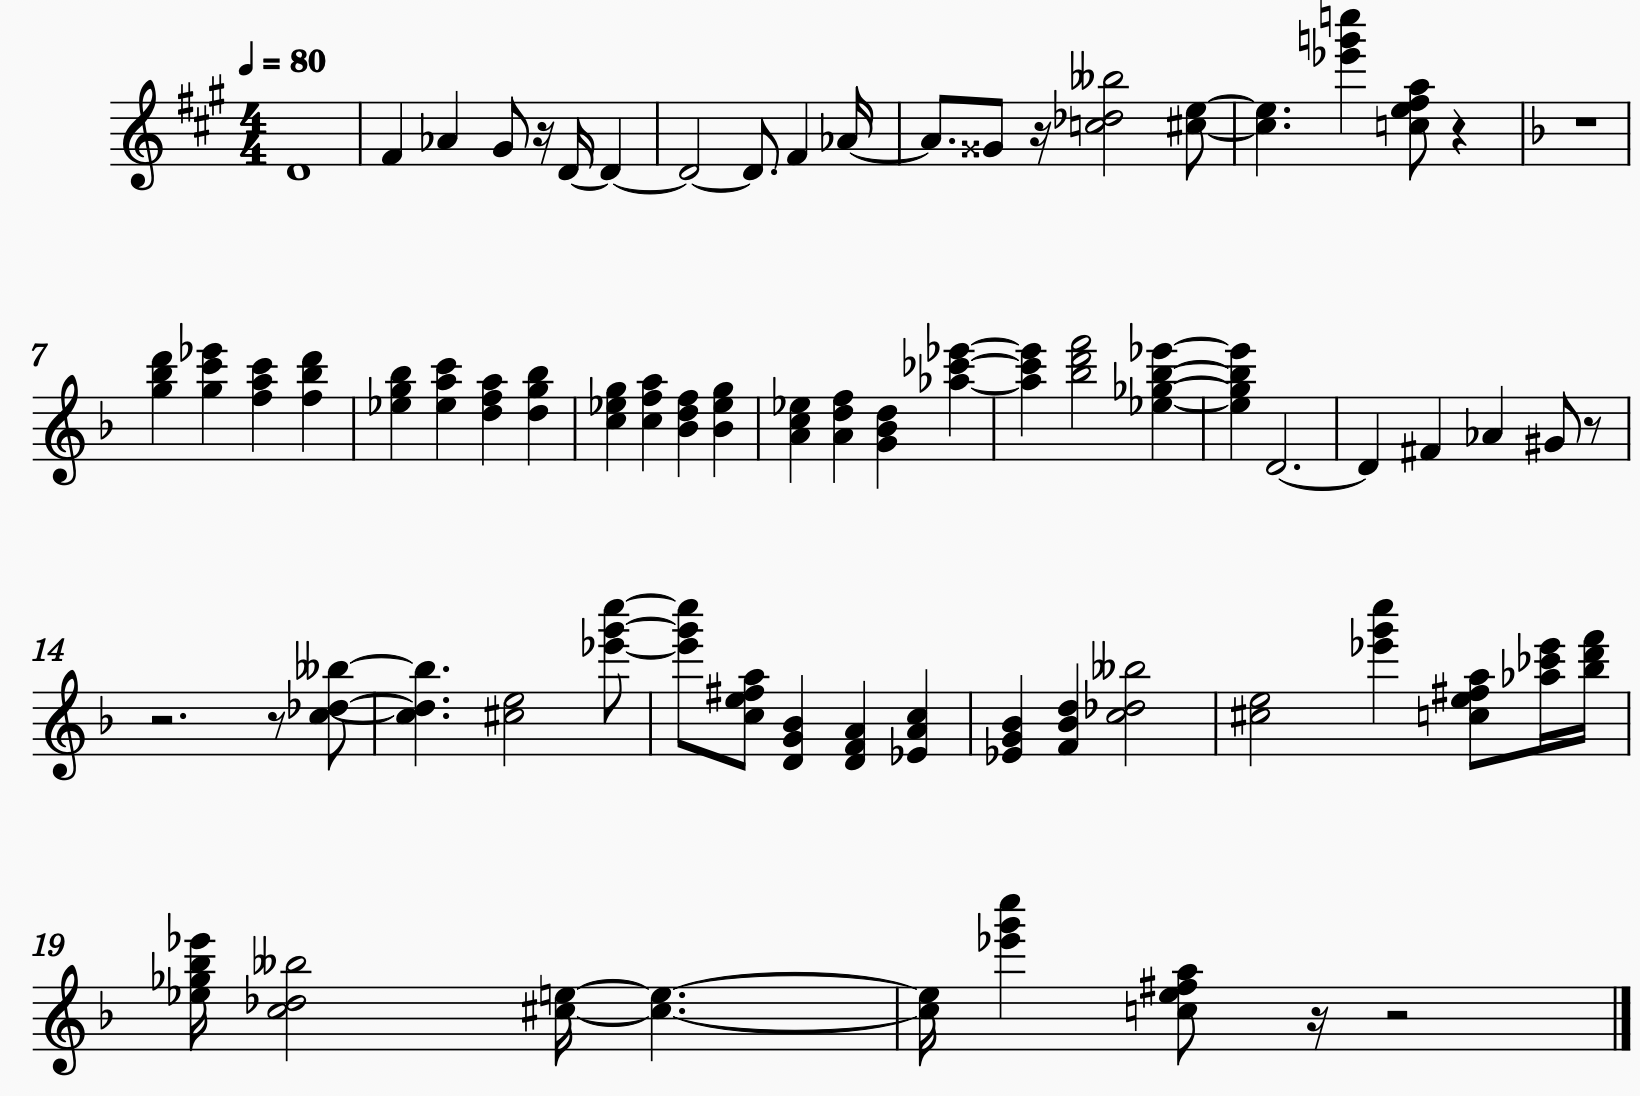
\includegraphics[width=\textwidth]{images/program1}
  %\caption{}
\end{figure}

%--------------------------------------------------------------------------------------------------------------------------------------------------------
\chapter{Future Work and Conclusion}
\section{Future Work}
Ideally, in the future MusAssist would support more complex musical states and elements including custom time signature and mid-composition time signature changes (similar to the behavior currently implemented for key signatures), clef changes within a part, multiple-clef parts (i.e. piano), multiple voicing within a part, custom parts (i.e. instruments), and multiple parts. Custom and changeable time signature would allow for the users to experiment with metric modulation, something that is currently impossible with the fixed common time setup. Clef changes within a part, both manual and automatic when a note extends too many ledger lines beyond a clef, would allow the score to be more nicely formatted and readable for the user. Support for two-clef piano would allow the MusAssist compiler to successfully modify how it generates cadences and harmonic sequences to include the essential baseline, in addition to the harmonization already implemented. Multiple voicing would allow for the user to create more complex musical lines, particularly with counterpoint. The latter two goals (custom parts and multiple parts) are somewhat outside MusAssist's goal as a music compositional aid, as this extends beyond the realm of music theory. However, users may enjoy this increased flexibility when composing. Finally, in line with its goal of offering the user complex musical templates, it would be ideal for MusAssist to provide support for key modulation; e.g. generating a sequence of chords that successfully modulates from one key to another key.
%--------------------------------------------------------------------------------------------------------------------------------------------------------
\section{Conclusion}
MusAssist is an external DSL whose Haskell-based compiler translates it to MusicXML that can be loaded into a major music notation software for further editing. Its syntax is simple and models the flow of thought a composer would have when writing music by hand. MusAssist fills a unique niche in the realm of musical DSLs by serving as a music compositional aid that allows the user to write specifications for complex musical templates at the levels of abstraction of the musical structures they describe. MusAssist is not intended to allow to the user to write a fully expressive musical piece, but rather to more easily create musical expressions that would be tedious to write by hand. For this reason, the output MusicXML file of a compiled MusAssist program is intentionally editable, rather than a static PDF format like a language such as LilyPond generates. MuseScore can be further valuable as an education tool to music theory students, allowing them to visualize musical structures from the definitions that they describe in MusAssist.

Clearly, DSLs are a powerful mechanism to push the boundaries of  computational creativity in the field of music. Scholars such as  Ge Wang continue to lead  research in institutions such as Stanford's CCRMA (Center for Computer Research in Music and Acoustics). By continuing to examine the creative expressive power of DSLs  in  music, we can continue to increase our understanding of the creative capabilities and extent of customization possible for  a programming language.

\bibinput{referencesexercisebib} 
\bibliography{referencesexercisebib}
\bibliographystyle{abbrvnat}

\end{document}